\chapter{Tribal NeuroSim - Futtatások, validáció és értelmezés}

\section{Világ-mechanikák és térbeli szubsztrát}
\label{sec:neurosim-26-mechanics}
% ==========================================================================

\subsection*{Hex-rácsvilág és biome-ok}

A szimuláció terét egy hexagonális rács alkotja, amelyben minden tile-nak legfeljebb hat szomszédja van. Ez a topológia egy térbeli gráf: a törzsek terjeszkedési útjai és stratégiai határai a szomszédsági reláción alapulnak, amelynek elvi háttere a 12-13.~fejezetekben tárgyalt pathfinder-architektúrában gyökerezik; itt a rács kizárólag mint szimulációs szubsztrátum kerül bemutatásra.

A világ mérete adatkészlet-függő. A flexset adatkészletből inicializált futtatások $\approx$36\,100 tile-os térképen játszódnak, mivel a Flex Queue klaszterpopuláció nagyobb és geográfiailag szétszórtabb. A SoloQ futtatások kisebb világokat kapnak; a vizsgált két SoloQ futtatás végső győztes területe 6\,356 és 9\,748 tile volt. Ez sűrűbb kezdeti törzsközeli elhelyezkedést és gyorsabb korai konszolidációt eredményezhet - amint az a~\ref{fig:neurosim-sq7777-tick301} ábrán is látható.

Minden tile-hoz egy biome-típus van rendelve, amely meghatározza az alap élelmiszertermelési rátát és mozgási tulajdonságokat:

\begin{table}[h]
\centering
\caption{Biome-típusok és élelmiszertermelési jellemzőik}
\label{tab:biomes}
\begin{tabular}{lll}
\hline
\textbf{Biome} & \textbf{Termelési szint} & \textbf{Különleges tulajdonság} \\
\hline
DenseForest & Magas        & Alapbiome; stabil élelmiszer-alap \\
Riverland   & Közepes      & Halászati bónusz ($+25\%$ folyóval szomszédos tile-okra) \\
DrySteppe   & Alacsony     & Alacsony foglalási költség, gyors terjeszkedés \\
Mountains   & Nulla        & Áthatolhatatlan - természetes terjeszkedési barrier \\
Marsh       & Alacsony     & Mozgásgátló, magasabb foglalási költség \\
Cold        & Nagyon alacsony & Populáció-fenntartás kritikus szint közelében \\
\hline
\end{tabular}
\end{table}

A biome-ok nem csupán passzív háttér: a törzs A\_resource artifaktuma közvetlenül modulálja, hogy mennyire hatékonyan tudja kiaknázni az adott biome potenciálját. Egy alacsony A\_resource értékű törzs DenseForest tile-on is szuboptimálisan teljesíthet, míg egy magas A\_resource értékű törzs DrySteppe-en is fenntartható szinten maradhat - bár ez utóbbi esetben a terjeszkedési kényszer szinte elkerülhetetlen.

\begin{figure}[h]
\centering
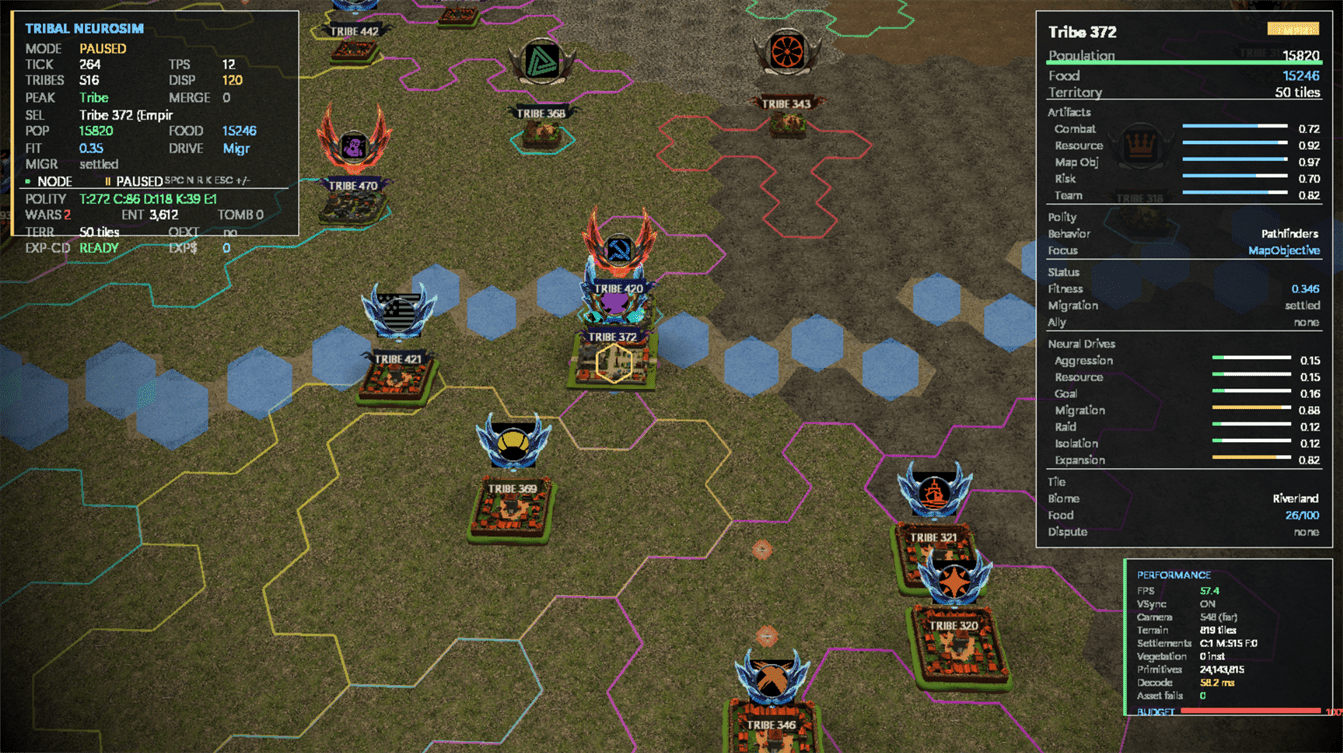
\includegraphics[width=0.9\textwidth]{assets/neurosim/run67fl7777-fl-s7777-tick264-firstempire.png}
\caption{Flexset, seed=7777, tick=264: közeli nézet a hex-rácson. Tribe~372 tile-jai körül biome-váltás (Riverland → DenseForest) látható; az egyes tile-ok élelmiszertermelési kapacitása biome-specifikus.}
\label{fig:neurosim-fl7777-tick264}
\end{figure}

\begin{figure}[h]
\centering
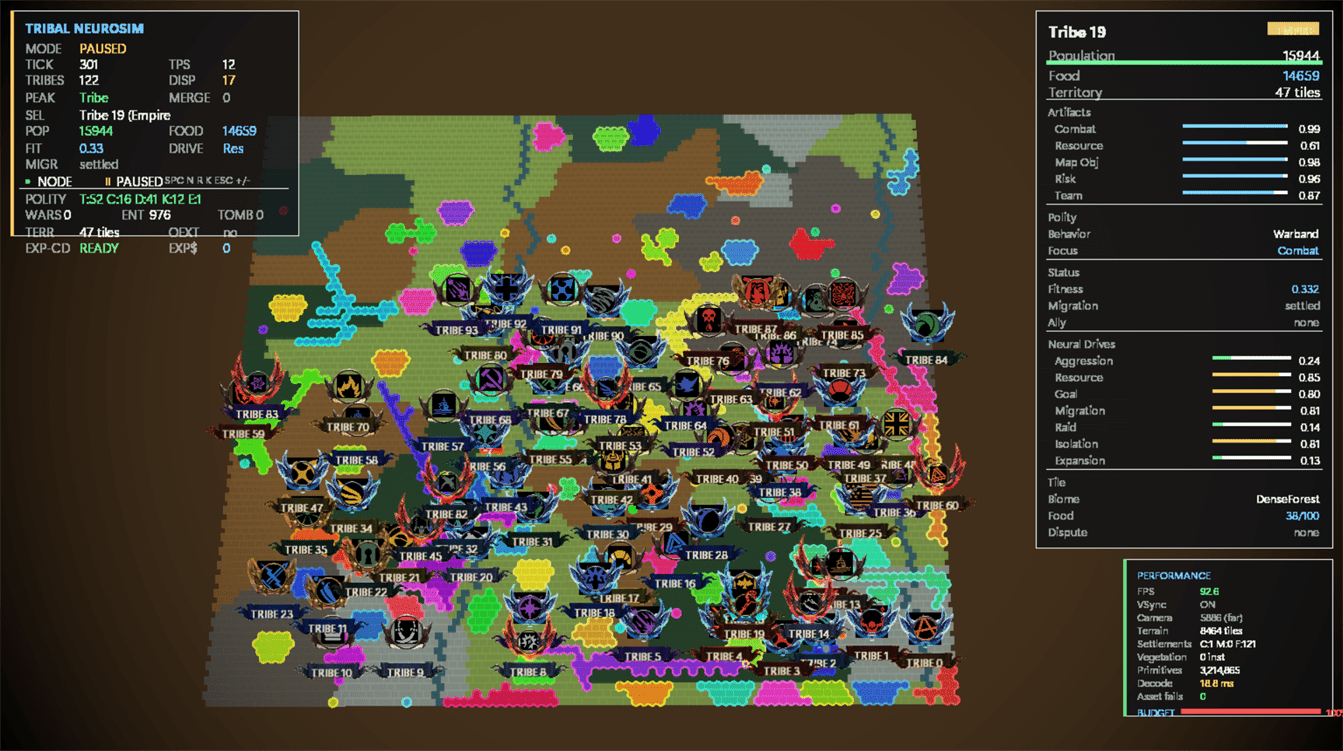
\includegraphics[width=0.9\textwidth]{assets/neurosim/run67sq7777-sq-s7777-tick301-firstempire.png}
\caption{SoloQ, seed=7777, tick=301: a kisebb soloq világ sűrűbb kezdeti elhelyezkedést és gyorsabb korai konszolidációt eredményez.}
\label{fig:neurosim-sq7777-tick301}
\end{figure}

\subsection*{Tile-tulajdonlás, vitatott zónák és terjeszkedési költség}

A v3-as architektúra bevezette a törtrészes tile-irányítás modelljét (TaskR4, 2026-05-06). Az egyes tile-ok nem bináris „1 vagy 0" alapon kerülnek hozzárendelésre; egyszerre több törzs is fennhatóságot tarthat rajtuk, törtrészes arányban, amelyet egy kompakt Rust adatstruktúra tárol:

\begin{lstlisting}[language={}, caption={Tile-irányítás adatstruktúra (részlet, TaskR4)}]
struct TileControl {
    tribe_id: u32,
    control_percentage: f32,  // pl. 0.70 = 70%-os irányítás
}
// Legfeljebb 4 törzs per tile, memóriahatárral
tile_occupants: Vec<ArrayVec<TileControl, 4>>
tile_is_disputed: Vec<bool>
\end{lstlisting}

\textbf{A vitatott zóna mechanikája:} ha két vagy több törzs ugyanazon a tile-on osztozik, a tile \textit{Disputed} státuszba kerül, és azonnali $-40\%$-os hatékonysági büntetés lép életbe minden ott végzett műveletre. A nettó erőforrás-hozam:

\begin{equation}
\text{nettó\_hozam} = \text{control\_percentage} \times (1{,}00 - 0{,}40)
\end{equation}

Ha például egy törzs egy vitatott tile-on 70\%-os irányítást tart fenn, a tényleges hozam $0{,}70 \times 0{,}60 = 0{,}42$, vagyis 42\%. Ez a matematikai kényszer természetes \textit{casus bellit} kelt: a törzs neurális hálózatának folyamatosan értékelnie kell, hogy a büntetett hozam elegendő-e a fennmaradáshoz, vagy erőszakos feloldásra van szükség.

A vitafeloldás három úton lehetséges, amelyeket a szimuláció 30 tickenként futtat: (1) \textit{passzív elfogadás}, ha az A\_risk artifaktum értéke $> 0{,}70$ és a büntetetett hozam meghaladja a túlélési küszöböt; (2) \textit{katonai fenyegetés}, ha az A\_combat értéke $> 0{,}80$ és magasabb, mint az ellenfélé - ekkor az ellenfél kénytelen visszavonulni; (3) \textit{diplomáciai fuzionálás}.

A terjeszkedés sebességét és költségét a TaskR8 (2026-05-07) implementáció rögzíti.
Minden foglalást egy per-törzs 25 tickes visszaszámlálás korlátoz; az igénylés csak
akkor hajtható végre, ha a következő két feltétel egyszerre teljesül:

\begin{equation}
\text{pop} \geq 80 + 25 \times |\mathcal{T}_i|
\quad \text{és} \quad
\text{food} - \text{cost}(\text{tile}) \geq 50
\end{equation}

ahol $|\mathcal{T}_i|$ az $i$-edik törzs jelenleg irányított tile-jainak száma,
a $\text{cost}(\text{tile})$ az adott biome foglalási költsége.
Újonnan foglalt tile-ok 75 tickes integrációs perióduson mennek keresztül,
amelynek során a hozam lineárisan emelkedik:

\begin{equation}
h(t) = h_{\max} \cdot \frac{t - t_0}{75}, \quad t_0 \leq t \leq t_0 + 75
\end{equation}

ahol $h_{\max}$ a biome nominális hozama és $t_0$ a foglalás tick-je.
Overextension akkor lép fel, ha az irányított tile-ok száma meghaladja
a fenntartható korlátot:

\begin{equation}
|\mathcal{T}_i| > 1 + \left\lfloor \frac{\text{pop}}{120} \right\rfloor
\quad \Rightarrow \quad \Delta\text{cost} = +10 \text{ egység/foglalás}
\end{equation}

\subsection*{Populáció és erőforrásmodell}

A törzs populációja és élelmiszer-készlete tickenként kölcsönösen hat egymásra. Az élelmiszerfogyasztás arányos a populációval; ha a fogyasztás meghaladja a termelést, az éhhalál mechanizmusa csökkenti a populációt. A \textit{resource\_drive} hajtóerő - amelynek értelmezése a 23.2.~alszekciójában kerül kifejtésre - modulálja a gyűjtési rátát: magas értékű törzsek aktívabban keresnek élelmiszer-forrást, alacsony értékű törzsek a harci vagy migrációs prioritások miatt elfogadják az alacsonyabb gyűjtési hatékonyságot.

A fenntartható egyensúly feltétele:
\begin{equation}
\text{populáció} \times \text{fogyasztás/fő} \;\leq\; \text{terület} \times \text{biome\_ráta} \times A\_\text{resource}
\end{equation}

Ha ez a feltétel hosszabb ideig sérül, a törzs elveszíti terjeszkedési képességét, majd - az éhhalál spiráljában - a fennmaradási képességét is. A szimuláció egyik fő szelekciós nyomása tehát nem a harci erő, hanem az erőforrás-egyensúly fenntartása.

\subsection*{Harci mechanika}

Minden háborús ticken Poisson-elosztású harci körök zajlanak le. Az eredményt az ütköző felek A\_combat artifaktumainak összevetése határozza meg: a magasabb harci profil magasabb valószínűséggel kényszeríti vissza az ellenfelet a magtile-okra. A háború három feltétel bármelyikének teljesülésével érhet véget: (1) az egyik fél összes tile-ját visszafoglalják és a törzs megsemmisül; (2) az egyik fél visszahúzódik a magtile-okra és megszűnik szomszédos lenni az ellenféllel; (3) mindkét fél a saját területére szorul - ekkor tüzszünet lép életbe.

A Poisson-elosztású harci körök matematikai modellje:

\begin{equation}
P(k \text{ találat}) = \frac{\lambda^k e^{-\lambda}}{k!},
\quad \lambda = a_{\text{att}} \cdot n_{\text{tiles}} \cdot 0{,}02
\end{equation}

ahol $a_{\text{att}}$ a támadó A\_combat artifaktuma, $n_{\text{tiles}}$ a
kontaktus-tile-ok száma, és a $0{,}02$ az alap harci szorzó.
A várható veszteség ezért $\mathbb{E}[k] = \lambda$; magas A\_combat és széles
kontaktzóna esetén a veszteség gyorsabban akkumulálódik, ami statisztikailag
előbb vezet teljes elfoglaláshoz, mint tárgyalásos visszavonuláshoz.
Ez magyarázza, miért végződik a legtöbb háború totális elfoglalással, nem
tűzszünettel: a Poisson-folyamat nem konvergál a halasztáshoz.

Az opportunista raid mechanizmus (raid\_drive $\times$ opportunity\_score $>$ küszöb) lehetővé teszi, hogy egy törzs akkor is háborút kezdeményezzen, ha még nem ért el katonai fölényt - például ha az ellenfél éppen más fronton harcol. Ez az algoritmus közvetlen felelős a 23.4.~alszekciójában bemutatott kaszkádjelenségekért: a flexset seed=7777 futtatás tick=2040-es Totális Háborújában 64 egyidejű opportunista háború indult, és a tick=2050-nél mért 63 élő törzsből tick=2250-re már csak 13 maradt.

A harci körök kimenetének statisztikai következménye, hogy a legtöbb háború
totális elfoglalással végződik, nem tűzszünettel. A Poisson-folyamat nem
konvergál az egyensúlyi megosztáshoz: ha $\lambda > 0$ fennáll minden harci
tick-en, a kumulált veszteség előbb-utóbb az egyik fél teljes összeomlásához
vezet. Mérsékelt $A_{\text{combat}}$ különbség esetén ez 50--200 tick-et vesz igénybe;
nagy különbség esetén (pl. 0{,}98 vs.\ 0{,}45) 10--30 tick is elegendő.
Ez a mechanika a szimuláció egyik erős kaosz-faktora: a látszólag stabil
kétpólusú helyzet megtörhet, ha egy harmadik törzs opportunista háborút indít
miközben az egyik fél már harci veszteséget szenved el.

\subsection*{Polity-szintek és fejlődési feltételek}

A törzsek hierarchikus politikai entitásokká fejlődhetnek, ha egyszerre teljesítik a populációs, területi és neurális küszöbfeltételeket. A fejlődési lépcsőfok:

\begin{table}[h]
\centering
\caption{Polity-szintek és közelítő fejlődési feltételek}
\label{tab:polity}
\begin{tabular}{lllll}
\hline
\textbf{Szint} & \textbf{Populáció} & \textbf{Terület} & \textbf{goal\_drive} & \textbf{Megjegyzés} \\
\hline
Tribe   & $\geq 80$    & $\geq 1$ tile    & -              & Kezdeti állapot \\
City    & $\geq 200$   & $\geq 5$ tile    & $> 0{,}40$     & Első settlement nyílik \\
Duchy   & $\geq 500$   & $\geq 15$ tile   & $> 0{,}55$     & Regionális dominancia \\
Kingdom & $\geq 1200$  & $\geq 40$ tile   & $> 0{,}65$     & Fuzionálási képesség \\
Empire  & $\geq 3000$  & $\geq 100$ tile  & $> 0{,}75$     & Végső győzelmi státusz \\
\hline
\end{tabular}
\end{table}

A settlement modell a polity szinthez kötött: minden szintlépés egy-egy settlement-csomópontot nyit meg a vizuális felületen. A MonoGame HUD-ban például a \textit{C1 M0 F12} jelölés azt jelenti, hogy az adott törzs 1 várossal, 0 erőddel és 12 farmmal rendelkezik - ezek a fejlettségi mutató közvetlen leolvasási pontjai. A settlement-szám egyszerre tükrözi a polity szintet és az erőforrás-infrastruktúra méretét.

\subsection*{Szövetség, fuzionálás és kihalás}

A diplomácia bináris, amint azt a 23.4.~alszekció részletezi: vagy teljes háború, vagy kölcsönös szövetség, esetleg fuzionálás. Szövetség esetén a felek megnemtámadási jelzést adnak a neurális bemenetükre, de önállóak maradnak - a \textit{legközelebbi\_szövetséges\_távolsága} bemeneti jel csökken, ami alacsonyabb isolation- és magasabb csapatkoordinációs nyomást jelent. A javított futásokban ezek a formális szövetségek ritkák: a rendszer inkább abszorpciós végjátékot produkál, ahol a nagyobb törzs ellenállással vagy ellenállás nélkül olvasztja be a kisebbet. Fuzionálás feltétele mindkét félnél: goal\_drive $> 0{,}55$, egyik sem áll éppen háborúban, és isolation $< 0{,}75$. Fuzionáláskor a két genomot fitnesz-súlyozott örökléssel vonják össze (lásd 23.3.~alszekció).

Kihalás esetén a törzs összes tile-ját visszafoglalják, majd tombstone rekord rögzíti az utolsó állapotot: genomot, leszármazást, harci rekordot és a kihalás okát. A leszármazási DAG - ahol minden törzs szülői linkeket tárol, nem teljes ancestry stringeket - technikailag egy irányított aciklikus gráf. A hex szomszédosság és a leszármazási lánc egyaránt gráf-struktúra; mindkét fogalom elvi háttere a 12-13.~fejezetekben kerül kifejtésre; itt kizárólag a szimulációs tartományra vonatkozó mechanikai alkalmazásuk releváns.

% ==========================================================================
\section{Iteratív újratervezés és hibaelőzmények}
\label{sec:neurosim-26-redesign}
% ==========================================================================

A Tribal NeuroSim v3-as, thesis-érett formája nem egyetlen tervezési iterációban jött létre. A rendszer jelenlegi állapota több prototípusgeneráció tanulságain, kritikus újratervezési döntéseken és célzott hibajavítási ciklusokon keresztül alakult ki. Ez az alszekció dokumentálja a korai verziók meghibásodásait, az ezekre adott architektúrális válaszokat és a liveness-fix során azonosított specifikus numerikus hibákat - mindezek nélkül a v3 futtatások validitása nem értelmezhető.

\subsection*{V1/V2 webes prototípus hibái}

A rendszer első, böngészőalapú prototípusa (v1/v2) egy React/Node frontend és egy Rust backend kombinációjaként futott, WebSocket streamen keresztül. Az első teljes futtatás post-mortem dokumentuma kilenc klinikai fázist azonosított, amelyek együttesen kritikus architektúrális hiányosságokat jeleztek.

\textbf{Inicializációs hiba (tick=21):} Az 599 törzs négy sűrű sorban jelent meg a térkép egy szűk sávjában; az élelmiszer-spawn rutin nem futott le. Minden törzs éhezési állapotban inicializálódott.

\textbf{Szellemháborúk (tick=257):} A harci állapotgép nem zárta le a befejezett háborúkat. Tick=257-re 323 aktív háború volt nyilvántartásban, miközben a teljes populáció ennél jóval kisebb volt - statisztikailag lehetetlen szám. Tick=3085-re egyetlen élő törzs maradt, mellette 182 aktív szellemháborúval. A probléma mélyebb oka az volt, hogy nem létezett strukturált háborúlezárási esemény: a háborús rekordok soha nem kaptak „lezárt" státuszt, ezért a rendszer mindet aktívnak tartotta. Ahogy a 22.3.~alszekció tárgyalja, az eseménybusz hiánya tette ezt a hibát láthatatlanná - a tick=187-es tömeges kihalásnak semmi nyoma nem maradt a naplóban.

\textbf{Migrációs státuszblokkada (tick=342-832):} A törzs állapotgépe „Migrating" státusba kerülhetett anélkül, hogy a tényleges térbeli koordinátái változtak volna. A heurisztikus célpont-keresés minden szomszédos tile-t egyenlőnek értékelt (élelmiszer=0 mindenhol), így az A* útkeresés null utat adott vissza, és a törzs helyben maradt. Tick=342-re a túlélő törzsek ~90\%-a migrációs állapotban volt, tényleges mozgás nélkül. Tick=832-re az éhhalál megsemmisítette a populáció döntő részét.

\textbf{Memóriaszivárgás (tick=2842):} A meghalt törzsek aktív objektumként maradtak a memóriában, azok állapotát a garbage collector nem szabadította fel. Tick=2842-nél a böngészőfelület teljesen megfagyott - a szimulációs vezérlők (pause, god-mode) nem reagáltak. A futtatás tick=3085-nél ért véget, egyetlen életben maradt törzs 3. generációs elérésével.

\subsection*{Kritikus újratervezési döntések}

A post-mortem analízis öt architektúrális döntést tett kötelezővé:

\begin{enumerate}
  \item \textbf{Rust authority:} A teljes szimulációs logika Rust-ba kerül. A frontend kizárólag renderelési kliens - nem fut szimulációt, nem tárol érdemi állapotot.
  \item \textbf{Kötelező eseménybusz:} Minden állapotátmenet strukturált eseményt bocsát ki, append-only naplóba. A végső térképállapot önmagában nem bizonyíték - az audit trail kötelező.
  \item \textbf{Tombstone ledger:} Minden kihaló törzs tombstone rekordot kap (kihalási ok, utolsó genom, leszármazás, utolsó populáció és területszám). A szellemháborúk megszüntetésének feltétele, hogy a halál pillanatában az összes aktív háborúra \textit{WarCancelled} esemény kerüljön.
  \item \textbf{Területi modell overhaul:} Bináris tile-tulajdonlás helyett törtrészes irányítás (lásd 24.1.~alszekció), vitatott zónák és terjeszkedési költségmodell.
  \item \textbf{MonoGame desktop kliens:} A böngésző prototípus memóriaszivárgásra hajlamos; a MonoGame C\# kliens FrameV1 bináris protokollon csatlakozik a Rust szerverhez, determinisztikus tick-szinkronnal.
\end{enumerate}

Ezek mellé két gameplay-szintű javítás is bekerült: az \textit{opportunista háborúmechanizmus} (raid\_drive × opportunity\_score alapú küszöb) és a \textit{stagnálási háborúmechanizmus} (ha N ticken nincs háborús aktivitás, nyomás épül fel), amelyek együttesen megakadályozzák a békés genomiális deadlock kialakulását - azt a jelenséget, amelynél minden törzs izolálódik és a szimuláció nem konvergál győztesre.

\subsection*{Task futtatási összefoglaló}

A v3-as rendszer implementációja diszkrét task-futtatásokon keresztül zajlott. Az alábbi táblázat összefoglalja a thesis szempontjából releváns feladatokat:

\begin{table}[h]
\centering
\caption{Implementációs task összefoglaló - kiemelt v3 futtatások}
\label{tab:tasks}
\begin{tabular}{llp{8cm}}
\hline
\textbf{Task} & \textbf{Dátum} & \textbf{Fő változás} \\
\hline
TaskR1 & 2026-05-06 & LineageRegistry (DAG ID rendszer); seed-entitás regisztráció; O(1) szülőlánc-lekérdezés \\
TaskR2 & 2026-05-06 & TombstoneLedger; ghost-war javítás (\textit{WarCancelled} státusz); halott törzsek ~100 byte-os rekordra csökkentve \\
TaskR4 & 2026-05-06 & Törtrészes tile-irányítás; \textit{TileControl} struktúra; vitatott zóna $-40\%$ büntetés \\
TaskR7 & 2026-05-06 & FrameV1 bináris protokoll; TNS3 envelope; little-endian; tile, háborús és esemény-delta szekciók \\
TaskR8 & 2026-05-07 & Hex-távolság; tereptől függő foglalási cost; overextension büntetés; 75 tickes integrációs periód \\
TaskM1 & 2026-05-08 & C\# FrameV1 dekóder; TNS3 envelope-parsírozás; backward-compatible V0 fallback \\
TaskM3 & 2026-05-08 & Hat-élű pointy-hex geometria; territory border rendering; Civ6-stílusú határvonal és crosshatch \\
TaskM9 & 2026-05-10 & MonoGame integráció; leszármazási inspektor panel (L); tombstone panel (K); HUD panelek \\
\hline
\end{tabular}
\end{table}

\subsection*{Liveness-fix részletei}

Az első teljes v3 futtatás (2026-05-14, 0-777 tick) statikusnak bizonyult: 599 törzs egyike sem halt meg, egyetlen háború sem zárult le, minden törzs pontosan 1 tile-t tartott fenn. A diagnózis három egymást erősítő hibát tárt fel.

\textbf{1. Kétszeres normalizálás:} A \textit{server.js} már 0-1 közé normalizálta az artifaktum-értékeket (osztás 4,5-tel vagy 5,0-val). A Rust \textit{TribeStats::from\_profile} ezután ismét 10-zel osztott, így az értékek 10$\times$ kicsik lettek. Az A\_combat értéke $\approx 0{,}03$ volt $0{,}3$ helyett. A harci veszteség: $0{,}03 \times 6000 \times 0{,}02 = 3{,}6$ egység/forduló - ekkora kár mellett egyetlen törzs sem halhatott meg háborúban. A javítás: az extra osztás eltávolítása.

\textbf{2. Migrációs oszcilláció:} A migrációs override azonnal aktiválódott minden \textit{Settling} vagy \textit{Foraging} állapotban lévő törzsre, amelynél migration\_drive $> 0{,}55$ és aggression $< 0{,}55$. Ez végtelen ciklust okozott: Settling → Migrating (0 tick után) → célpont elérve → Settling → azonnal Migrating. A törzsek ~15\%-a soha nem töltötte el a \textit{apply\_territory\_expansion} által megkövetelt minimális időt \textit{Settling} állapotban, ezért nem igényelt tile-okat. Javítás: \textit{ticks\_in\_state >= 15} feltétel hozzáadása a migrációs override elé.

\textbf{3. Terjeszkedési küszöb:} A terjeszkedési feltétel \textit{resource\_drive < 0.25} volt, ami a törzsek $\approx 63\%$-át kizárta a terjeszkedésből. A küszöb \textit{0.10}-re csökkentése után a törzsek $\approx 95\%$-a válhatott jogosulttá tile-igénylésre.

Az ezt követő \textit{post-first-run} javítási körben (2026-05-16) három további hiba javítása történt: (1) a kihaló törzsek tile-jai korábban semleges státuszba kerültek ahelyett, hogy a hódítóra szállnának; (2) az \textit{AtWar} állapotban lévő törzsek nem tudtak élelmiszert gyűjteni, így a nagy birodalmak éhhalálban pusztultak el ahelyett, hogy harci veszteség döntötte volna el a háborút - ez a \textit{starvation cascade} jelenség; (3) a valós flexset klaszterprofilok minden artifaktumon $0{,}89$-$0{,}99$ értékeket mutattak, ami viselkedési monokultúrát okozott: minden törzs \textit{Warband} archetípussal indult. A $[0{,}6, 1{,}0]$ véletlenszerű artifaktum-skálázás - determinisztikus, genome-seed alapú - megszüntette ezt.

\subsection*{Determinizmus-hiba visszautalása}

A 22.4.~szekcióban részletesen tárgyalt determinizmus-hiba - az SQLite-ból rendezés nélkül betöltött klasztersorrend véletlenszerűsége és annak javítása (\textit{clusters.sort\_by(|a, b| a.id.cmp(\&b.id))}) - szintén ebbe az iteratív újratervezési folyamatba illeszkedik. Az igazolás (CLI tick=100 és MonoGame tick=100 azonos kimenete: \textit{alive=593, City:41, Tribe:552}) a liveness-fix utáni állapotra vonatkozik, és a reprodukálható futtatások előfeltételét képezi.

% ==========================================================================
\section{A szimuláció teljes matematikai modellje}
\label{sec:neurosim-26-mathmodel}
% ==========================================================================

Ez a szekció a Tribal NeuroSim formális matematikai leírását adja. A cél nem a kód dokumentálása,
hanem annak megmutatása, hogy a rendszer mögött egységes, zárt matematikai struktúra áll --
amelynek minden komponense levezethető egymásból.

\subsection*{Állapottér}

A szimuláció állapota a $t$-edik ticken:
\begin{equation}
\mathcal{S}(t) \;=\; \Bigl(\, \mathcal{W},\;\bigl\{\mathcal{A}_i(t)\bigr\}_{i \in \mathcal{I}(t)},\;\mathcal{E}(t) \,\Bigr)
\end{equation}
ahol $\mathcal{W}$ a statikus hex-rácsvilág (biome-ok halmaza és szomszédossági reláció),
$\mathcal{I}(t) \subseteq \mathbb{N}$ az élő törzsek indexhalmaza a $t$-edik ticken,
és $\mathcal{E}(t)$ az eseménynapló állapota (append-only). Az egyes törzsek ágensállapota:
\begin{equation}
\mathcal{A}_i(t) \;=\; \bigl(\, g_i(t),\;\mathcal{T}_i(t),\; p_i(t),\; f_i(t),\;\boldsymbol{\alpha}_i,\;\sigma_i(t) \,\bigr)
\end{equation}
ahol $g_i(t)$ a törzs genomja (súlymátrix + topológia), $\mathcal{T}_i(t) \subseteq \mathcal{W}$
a tulajdonolt tile-ok halmaza, $p_i(t) \in \mathbb{N}$ a populáció, $f_i(t) \in \mathbb{R}_{\geq 0}$
az élelmiszer-készlet, $\boldsymbol{\alpha}_i = (a_c, a_r, a_m, a_k, a_t)^{\!\top} \in [0,1]^5$
az invariáns klaszter-derivált artifact-prior vektor, és $\sigma_i(t)$ az aktuális viselkedési
állapot.

\subsection*{Neurális döntéshozatal}

A törzs neurális hálózatának bemeneti vektora:
\begin{equation}
\mathbf{x}_i(t) \;=\; \bigl(\,
  \tfrac{f_i}{f_{\max}},\;
  \tfrac{p_i}{p_{\max}},\;
  \tfrac{|\mathcal{T}_i|}{T_{\max}},\;
  \rho_i,\;
  a_c,\; a_r,\; a_m,\; a_t,\;
  d^{\text{enemy}}_i,\; d^{\text{ally}}_i,\;
  a_k
\,\bigr)^{\!\top} \;\in\; [0,1]^{11}
\end{equation}
ahol $\rho_i \in [0,1]$ az éhhalál-közelség (\textit{feed risk}), $d^{\text{enemy}}_i$ és
$d^{\text{ally}}_i$ a normált hex-távolságok a legközelebbi ellenfélhez és szövetségeshez.
A neurális kimenet:
\begin{equation}
\mathbf{d}_i(t) \;=\; \tanh\!\Bigl( W_i(t)\,\mathbf{x}_i(t) \;+\; \mathbf{b}_i(t) \Bigr)
\;\in\; [-1,1]^7
\end{equation}
ahol $W_i(t)$ a genom súlymátrixa, $\mathbf{b}_i(t)$ a torzításvektor, és a kimenet hét
komponense sorban az \textit{aggression}, \textit{resource\_drive}, \textit{goal\_drive},
\textit{migration\_drive}, \textit{raid\_drive}, \textit{isolation} és \textit{expansion\_speed}
hajtóerők.

\subsection*{Erőforrás-dinamika}

Az élelmiszer-egyenleg egy tick alatt:
\begin{equation}
f_i(t+1) \;=\; f_i(t)
\;+\; \underbrace{\sum_{j \,\in\, \mathcal{T}_i(t)} r(j)\cdot c_{ij}(t)\cdot a_r}_{\text{gyűjtés}}
\;-\; \underbrace{p_i(t)\cdot\kappa}_{\text{fogyasztás}}
\end{equation}
ahol $r(j) \geq 0$ a $j$-edik tile biome-hozama, $c_{ij}(t) \in [0,1]$ az irányítási arány
(vitatott tile esetén $c_{ij}(t)\cdot(1 - \delta_{\text{dispute}})$ érvényes, ahol
$\delta_{\text{dispute}} = 0{,}40$), és $\kappa > 0$ az egy főre eső fogyasztási ráta.
Ha $f_i(t+1) < 0$, éhhalál következik be: $p_i(t+1) \leftarrow \max\bigl(0,\; p_i(t+1) + f_i(t+1)/\kappa\bigr)$.

A fenntartható egyensúly feltétele:
\begin{equation}
p_i(t)\cdot\kappa \;\leq\; a_r \cdot \sum_{j \,\in\, \mathcal{T}_i(t)} r(j)\cdot c_{ij}(t)
\end{equation}

\subsection*{Terjeszkedési feltételrendszer}

Egy új tile $j^* \notin \mathcal{T}_i(t)$ igénylése csak akkor hajtható végre, ha egyszerre
teljesül:
\begin{equation}
p_i(t) \;\geq\; 80 + 25\cdot|\mathcal{T}_i(t)|
\qquad \text{és} \qquad
f_i(t) - \mathrm{cost}(j^*) \;\geq\; 50
\qquad \text{és} \qquad
\Delta_i(t) = 0
\end{equation}
ahol $\Delta_i(t) \in \{0,1,\ldots,25\}$ a per-törzs foglalási visszaszámlálás. Overextension
akkor lép fel, ha $|\mathcal{T}_i| > 1 + \lfloor p_i/120 \rfloor$, és minden további
foglalási kísérlethez $+10$ egységnyi büntetőköltséget ad. Újonnan igényelt tile hozama
lineárisan integrálódik 75 tick alatt:
\begin{equation}
h_j(t) \;=\; r(j)\cdot\min\!\Bigl(1,\;\tfrac{t - t_0(j)}{75}\Bigr), \qquad t \geq t_0(j)
\end{equation}

\subsection*{Harci modell}

Két törzs, $i$ (támadó) és $j$ (védő), háborúja Poisson-folyamatként modellezett.
Egyetlen harci körben a védő vesztesége:
\begin{equation}
\Delta p_j \;\sim\; \mathrm{Poisson}(\lambda_{ij}), \qquad
\lambda_{ij} \;=\; a_{c,i}\cdot|\partial\mathcal{T}_i \cap \partial\mathcal{T}_j|\cdot\mu_{\text{combat}}
\end{equation}
ahol $a_{c,i}$ a támadó \textit{A\_combat} értéke, $|\partial\mathcal{T}_i \cap \partial\mathcal{T}_j|$
a kontaktzóna (szomszédos tile-párok száma a két terület határán), és $\mu_{\text{combat}} = 0{,}02$
az alap harci szorzó. A várható veszteség tickenként: $\mathbb{E}[\Delta p_j] = \lambda_{ij}$.
Magas $a_{c,i}$ és széles kontaktzóna esetén ez gyorsan vezet totális elfoglaláshoz, ami
magyarázza, miért végződik a legtöbb háború kapituláció formájában, nem tárgyalásos tűzszünettel.

\subsection*{Fitnesz és evolúciós operátor}

A törzs összetett fitnesz-értéke:
\begin{equation}
\phi_i(t) \;=\; w_1\cdot\frac{t_{\text{alive},i}}{t} \;+\; w_2\cdot\frac{|\mathcal{T}_i(t)|}{T_{\max}} \;+\; w_3\cdot\frac{p_i(t)}{p_{\max}} \;+\; w_4\cdot\frac{\pi_i}{4} \;+\; w_5\cdot\frac{n_{\text{won},i}}{n_{\text{won},i}+n_{\text{lost},i}+1}
\end{equation}
ahol $\pi_i \in \{0,1,2,3,4\}$ a polity-szint (Tribe=0, \ldots, Empire=4), $n_{\text{won},i}$
és $n_{\text{lost},i}$ a nyert és veszített háborúk száma, és $(w_1,\ldots,w_5)$ az összetevők
súlyai. A generációs határponton ($t \equiv 0 \pmod{1000}$) a mutációs ráta:
\begin{equation}
\mu_i \;=\;
\begin{cases}
2\mu_0 & \text{ha } r_i \leq 0{,}20 \\
\mu_0  & \text{ha } 0{,}20 < r_i < 0{,}80 \\
\tfrac{1}{2}\mu_0 & \text{ha } r_i \geq 0{,}80
\end{cases}
\end{equation}
ahol $r_i \in [0,1]$ a relatív fitnesz-rang és $\mu_0 = 0{,}05$ az alap mutációs ráta.
Fuzionáláskor az örökös genomja fitnesz-súlyozott keverék:
\begin{equation}
g_k \;=\; \frac{\phi_i\cdot g_i \;+\; \phi_j\cdot g_j}{\phi_i + \phi_j}
\end{equation}

\subsection*{Megállási feltétel és végső egyensúly}

A szimuláció megáll, ha:
\begin{equation}
|\mathcal{I}(t)| \;\leq\; 1
\end{equation}
A győztes törzs $k^* = \arg\min_{i \in \mathcal{I}(t)} |\mathcal{I}(t)|$ örökli az összes
tile-t: $\mathcal{T}_{k^*} \leftarrow \mathcal{W}$. Ez a feltétel az evolúciós szelekció
legélesebb formája: nincs részleges kimenetel, nincs tárgyalás, nincs megosztott győzelem.
Az egész rendszer egyetlen stabil állapotba konvergál, amelyet a matematikai struktúra
elkerülhetetlenné tesz.

% ==========================================================================
\section{Validációs filozófia és determinizmus-igazolás}
\label{sec:neurosim-26-validation}
% ==========================================================================

\subsection*{Validációs alapelvek}

A szimulációs kísérlet tudományos értéke nem abban áll, hogy a rendszer lefutott, hanem abban, hogy ellenőrizhető körülmények között, megismételhetően ugyanazt az eredményt produkálja. A Tribal NeuroSim validációs stratégiája három egymást erősítő elvből épül fel.

\textbf{Determinisztikus seed-ek.} Minden futtatás egy egész szám seed értékkel inicializálódik. Azonos seed és azonos adatkészlet esetén a szimuláció minden egyes törzsi döntést, minden háborús kimenetelt és minden kihalási eseményt ugyanabban a sorrendben reprodukál. Ez a tulajdonság teszi lehetővé, hogy futtatások között összehasonlítás legyen érvényes: ha két futttatás ugyanolyan seed-del, de eltérő adatkészlettel indul, a különbség egyértelműen az inicializációs klaszterprofilnak tudható be.

\textbf{Nem elegendő, hogy „lefutott".} A validáció feltétele, hogy az adott futtatás $N$-ből $N$ esetben azonos \textit{final\_summary} rekordot állítson elő - azonos győztes TribeId-vel, azonos polity-szinttel, azonos tombstone-számmal. Egy egyszeri futás, amelynek eredményét nem lehet megismételni, nem tekinthető empirikus bizonyítéknak; csupán egy megfigyelt eseménynek.

\textbf{Esemény-alapú értelmezés.} Minden törzs-viselkedésre vonatkozó állítás - hogy egy törzs opportunistán csapott le, hogy egy trilaterális háborúban koordinálatlanul vett részt, hogy sorozatos védelmi győzelmeket aratott - kizárólag a naplóbejegyzésekre épülhet. A végső térképkép önmagában nem bizonyít semmit: két különböző belső dinamika ugyanolyan területi végeredménnyel zárulhat. Az eseménybusz (lásd 22.3.~alszekció) és a JSONL naplók a forrásadatok; az értelmezések ezekből vannak levezetve.

\textbf{Amit a validáció nem bizonyít.} A reprodukálhatóság és az esemény-alapú igazolás nem egyenértékű azzal, hogy a modell valóság-konform. A szimuláció saját szabályain belül konzisztens; ezek a szabályok azonban nem a valódi emberi pszichológia vagy valódi LoL-meccs-dinamika leírásai. Az eredmények nem vihetők át közvetlenül valódi viselkedési előrejelzésekre. A győztes viselkedési archetípus meghatározásán azt értjük, hogy az adott konfiguráció ebben a szimulációban, ezekkel a paraméterekkel nyert - nem azt, hogy az adott stratégia objektívan fölényes.

% --------------------------------------------------------------------------
\subsection*{F2 korai futtatás - mit lehet belőle megtartani}
% --------------------------------------------------------------------------

Az F2 futtatás a fejlesztés egyik korai, auditált állapota volt. Hasznos marad,
mert megmutatta, hogy az összes neurális kimenet aktív, a fitneszfüggvény elkezdte
szétválasztani a törzseket, és a szimuláció már nem statikus térképanimációként
viselkedett. Nem helyes azonban végleges bizonyítékként kezelni: a későbbi
post-first-run javítások után változott a tile-öröklés, a háború alatti
élelmiszergyűjtés, az artifact-diverzitás és a tombstone-audit részlete.

A futtatás paraméterei: 599 klaszter-derivált törzs, Flexset adatkészlet, 1200 tick, fejnélküli CLI mód, JSONL naplózás. Az összes neurális kimenet aktivitása igazolható a 23.2.~alszekció táblázatára visszautalva: mind a 7 kimenet minden 100 tickes ablakban jelen volt, egyetlen kimenet sem szaturált, és az értékkészlet egész végig 0,221 és 0,881 között mozgott.

A fitneszfejlődés adatai a törzsi differenciáció bizonyítékai:

\begin{table}[h]
\centering
\caption{Átlagos és maximális fitnesz alakulása az F2 korai futtatásban (1200 tick)}
\label{tab:f2-fitness}
\begin{tabular}{rlll}
\hline
\textbf{Tick} & \textbf{Átlag} & \textbf{Maximum} & \textbf{Szóródás (max - átlag)} \\
\hline
1    & 0,008 & 0,011 & 0,003 \\
100  & 0,070 & 0,240 & 0,170 \\
300  & 0,129 & 0,378 & 0,249 \\
600  & 0,172 & 0,424 & 0,252 \\
900  & 0,218 & 0,495 & 0,277 \\
1200 & 0,277 & 0,556 & 0,279 \\
\hline
\end{tabular}
\end{table}

A szóródás (átlag-maximum különbség) 0,003-ról 0,279-re nőtt. Ez nem egyenletes populációszintű növekedés: a fitneszfüggvény már ekkor szétválasztotta a sikeresebb és kevésbé sikeres törzseket. A kihalási ráta csúcsa a tick=900-999 ablakban volt (74 törzs/100 tick), az aktív háborúk száma pedig tick=800 körül érte el maximumát (~274 egyidejű háborúval).

Ezek az adatok azt támasztják alá, hogy az F2 ponton a neurális aktivitás és a fitnesz-differenciáció már jelen volt. A véglegesebb validációt viszont nem ez a futás adja, hanem a későbbi, javított szabályokkal készült determinisztikus logok.

\begin{figure}[h]
\centering
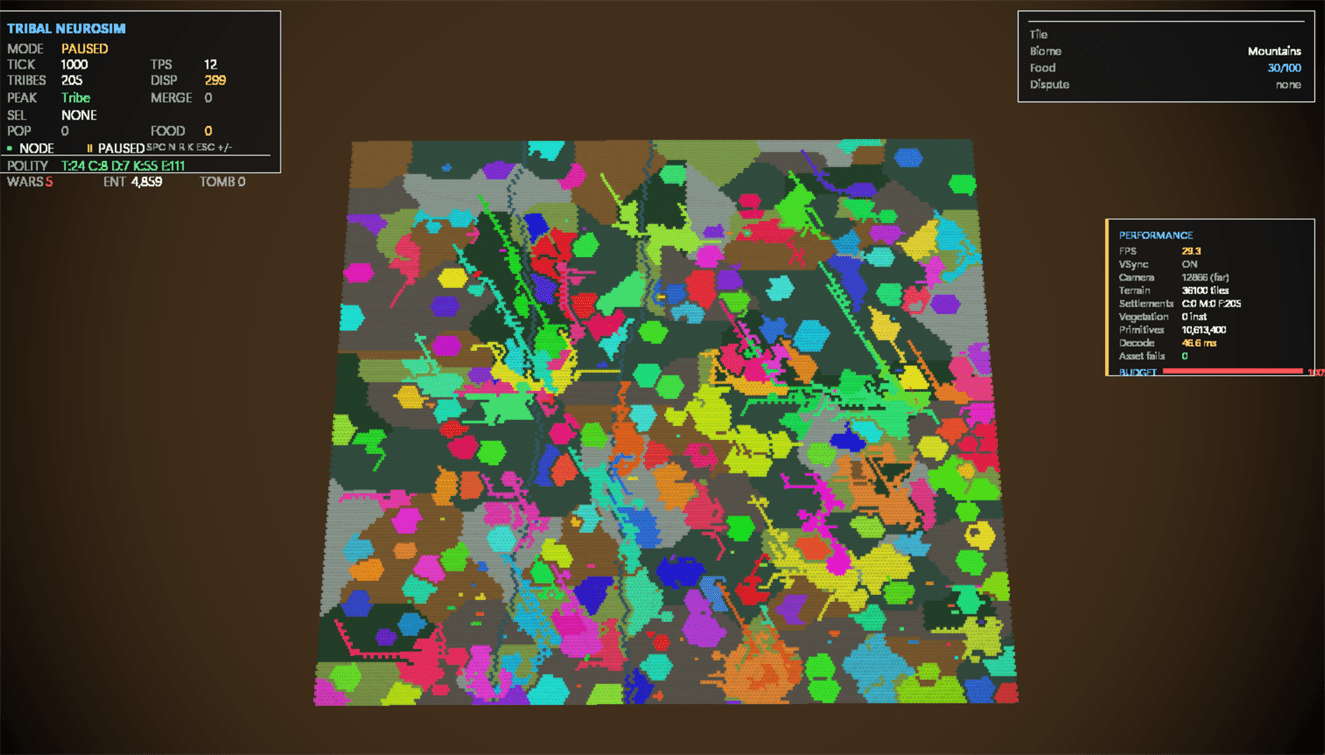
\includegraphics[width=0.9\textwidth]{assets/neurosim/run67fl7777-fl-s7777-tick1000.png}
\caption{Flexset, seed=7777, tick=1000: 205 élő törzs az F2 korai futtatással összevethető állapotban. Az összes polity-szint jelen van, a birodalom-korszak megkezdődött.}
\label{fig:neurosim-fl7777-tick1000}
\end{figure}

\begin{figure}[h]
\centering
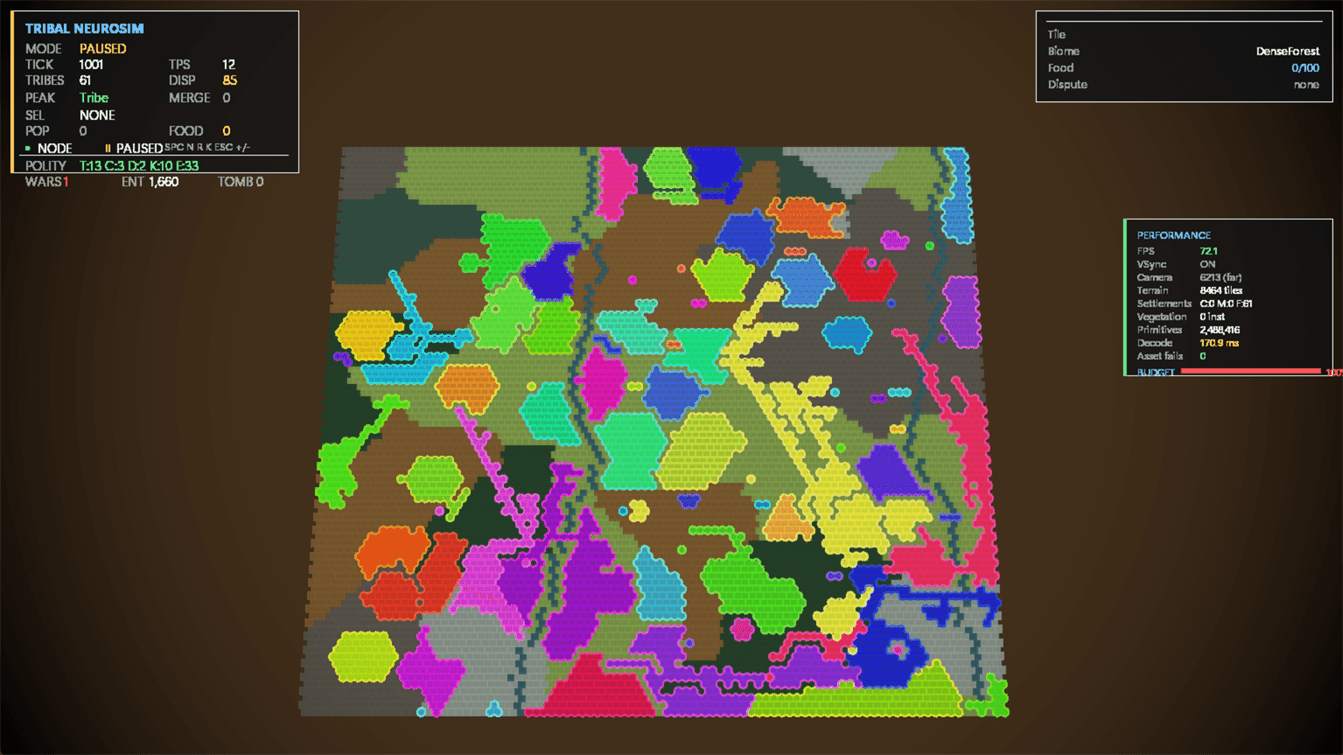
\includegraphics[width=0.9\textwidth]{assets/neurosim/run67sq7777-sq-s7777-tick1000.png}
\caption{SoloQ, seed=7777, tick=1000: 61 élő törzs, kisebb világ. Összehasonlításképpen: azonos tick-en a flexset futtatás 3,4$\times$ több entitást tartott életben - ez a két adatkészlet eltérő térbeli dinamikájának és kezdő törzsszámának közvetlen következménye.}
\label{fig:neurosim-sq7777-tick1000}
\end{figure}

% --------------------------------------------------------------------------
\subsection*{Javított determinisztikus futások}
% --------------------------------------------------------------------------

A 2026.~május~16-i post-first-run javítási kör után a validáció fókusza áthelyeződött:
nem az volt a kérdés, hogy a kimenetek aktívak-e, hanem az, hogy a teljes világ
visszaellenőrizhetően és determinisztikusan konvergál-e. Ebben a körben a kihalt törzsek
területe már öröklődött, az \textit{AtWar} állapot nem okozott éhhalál-kaszkádot,
az artifact skálázás megszüntette a Warband-monokultúrát, és a tombstone rekordok
alapító PUUID szinten is auditálhatóbbá váltak.

A 2026.~május~18-i Tribe 397 futás már ezt a javított állapotot dokumentálta. A teljes,
599 törzses világ egyetlen túlélőig konvergált, és a végállapot nem csak képből, hanem
eseménysorból is rekonstruálható volt: Tribe 397 több védelmi győzelem, opportunista
háború és végső direkt konfliktus után maradt életben.

\begin{table}[h]
\centering
\caption{Javított determinisztikus futás kiemelt pontjai (Tribe 397, 2026-05-18).}
\label{tab:tribe397-validation}
\begin{tabular}{rlp{7.2cm}}
\hline
\textbf{Tick} & \textbf{Állapot} & \textbf{Értelmezés} \\
\hline
50   & 557 élő törzs & korai terjeszkedés, még birodalmak nélkül \\
900  & 277 élő törzs & erős konszolidáció, 105 Empire \\
5000--6900 & hosszú plateau & kevés, nagy birodalom tartja egymást nyomás alatt \\
7650 & 2 élő törzs & Tribe 397 és Tribe 269 végjáték \\
7800 & 1 élő törzs & Tribe 397 győztes, 51\,391 tile kontroll \\
\hline
\end{tabular}
\end{table}

\begin{lstlisting}[language={},caption={Javított végállapot-részlet a Tribe 397 futásból}]
[SIM tick=7800] alive=1 tiles=51391 max_tile=51391 avg_pop=5305532 wars_active=0
\end{lstlisting}

Ez a futás erősebb thesis-szintű bizonyíték, mint az F2: nem csak azt mutatja, hogy
a neurális hajtóerők aktívak, hanem azt is, hogy a javított szabályrendszer mellett
a teljes eseménysor auditálható, a végső győztes rekonstruálható, és a modell nem
ragad be szövetségi vagy békés deadlockba.

% --------------------------------------------------------------------------
\subsection*{Batch determinizmus-ellenőrzés}
% --------------------------------------------------------------------------

A determinizmus-javítás (lásd 22.4.~alszekció) helyességét batch futtatásokkal igazoltuk. A \textit{run-batch.ps1} szkript képes $N$ párhuzamos fejnélküli futtatást azonos seed értékkel elindítani, és minden futtatás \textit{final\_summary} rekordját JSON-ként rögzíteni. Az ellenőrzés feltétele: mind az $N$ rekordban azonos \textit{TribeId} és azonos \textit{PolityBehavior} értéknek kell szerepelnie.

Két batch-ellenőrzés elvégzése igazolta a javítás helyességét:

\textbf{Flexset, seed=42}: öt párhuzamos fejnélküli futtatás mindegyikében Tribe 596 (Warband/Combat viselkedési archetípus) győzött. A győztes \textit{TribeId}, a \textit{winner\_tier} és a \textit{total\_ticks} értékek minden futtatásban bit-azonosak voltak.

\textbf{SoloQ, seed=7777}: a jelen fejezetben elemzett \textit{run67sq7777} teljes futtatási logja szerint Tribe 70 győzött, tick=2541-nél. Ez a konkrét kísérleti narratíva ezért Tribe 70-et tekinti a seed=7777 SoloQ futtatás győztesének.

\begin{lstlisting}[language={}, caption={Batch determinizmus-ellenőrzés parancssora}]
# 5 futtatas azonos seed-del, eredmeny JSONL-be
.\run-batch.ps1 -Runs 5 -Seed 42 -DatasetId flexset
# Kimenet: final_summary sorok mind azonos winner_id-t es behavior-t mutatnak
\end{lstlisting}

Ez az eredmény két dolgot igazol egyszerre: egyrészt hogy a \textit{clusters.sort\_by} javítás valóban megszüntette a véletlenszerű klasztersorrendből fakadó divergenciát, másrészt hogy a neurális hálózat és a szimulációs motor együttes viselkedése determinisztikus a teljes futtatás hosszán keresztül - nemcsak az első 100 tickre, amelyet a MonoGame-CLI összehasonlítás igazolt.

% --------------------------------------------------------------------------
\subsection*{Mit támogat a validáció - és mit nem}
% --------------------------------------------------------------------------

\textbf{A validáció alátámasztja az alábbi állításokat:}

\begin{itemize}
  \item A klaszter-derivált priorok mérhetően eltérő szimulált viselkedést produkálnak különböző adatkészletek esetén.
  \item A Flexset inicializáció mindkét tesztelt seednél azonos viselkedési kimenetelhez vezetett (Warband/Combat archetípus, alacsony agresszió, magas migráció); szisztematikus seed-sweep még nem készült el.
  \item A SoloQ inicializáció seedenként változékony viselkedési kimenetelt produkál.
  \item A futtatások reprodukálhatók: azonos seed és adatkészlet esetén a győztes és a teljes final\_summary rekord bit-azonos marad.
  \item A törzsi viselkedés esemény-naplókkal alátámasztható: minden állítás (kaszkádháborúk, trilaterális koalíciók, sorozatos védelmi győzelmek) konkrét JSONL-bejegyzésekre hivatkozik.
\end{itemize}

\textbf{A validáció nem bizonyítja az alábbiakat:}

\begin{itemize}
  \item Hogy a modell valóság-konform - a szimulációs szabályok közelítések, nem valódi emberi viselkedés leírásai.
  \item Hogy az eredmények átvihetők tényleges LoL-meccs kimenetelekre vagy valódi csapatdinamikára.
  \item Hogy a győztes viselkedési archetípus objektíven a legjobb stratégia - csupán annyi igaz, hogy a választott szabályok alatt, ebben a szimulációs környezetben nyert.
  \item Hogy a Flexset és SoloQ klaszterprofilok közötti különbség \textit{oka} a megfigyelt viselkedési divergenciának - a kapcsolat korrelatív, nem okozati.
\end{itemize}

Ez a határ nem gyengíti a kísérlet eredményét, hanem pontosítja a thesis-érvényes állítások körét: a Tribal NeuroSim demonstrálja, hogy gráf-derivált klaszterprofilok mérhetően eltérő emergáló dinamikát indítanak el azonos szabálykörnyezetben. Ez a demonstráció reprodukálható, inspektálható és esemény-alapon igazolt.

% ==========================================================================
\section{Kísérleti futtatási narratívák}
\label{sec:neurosim-26-runs}
% ==========================================================================

Ez a szekció a négy teljes kísérleti futtatást esemény-narratívaként mutatja be. A cél nem az, hogy a térképképeket önmagukban bizonyítékként kezelje, hanem hogy a futtatási naplókból származó tick-számokat, háborús eseményeket és végállapotokat értelmezhető kísérleti történetté rendezze. A konfliktusos szerkezetek értelmezésekor a 23.4.~alszekció táblázatában bevezetett típusokra hivatkozom vissza: a tömeges opportunista háborúk, a többfrontos nyomás és a végjátékbeli párharcok ugyanannak az eseménybusz-alapú mechanikának különböző megfigyelhető formái.

\subsection*{Flexset, seed=7777}

\begin{table}[h]
\centering
\caption{Flexset seed=7777 futtatás összefoglalója}
\label{tab:neurosim-run-fl7777-summary}
\begin{tabular}{ll}
\hline
\textbf{Mező} & \textbf{Érték} \\
\hline
Adatkészlet & flexset (EUNE Master+ Flex Queue) \\
Seed & 7777 \\
Indítótörzsek & 599 \\
Térkép & $\approx$36\,100 tile \\
Végső tick & 2538 \\
Győztes & Tribe 355 \\
Behavior / fókusz & Empire / Warband / Combat \\
Agresszió & 0,18 \\
Migráció & 0,88 \\
Kulcsesemény & Totális Háború, tick=2040: 64 egyidejű deklaráció \\
\hline
\end{tabular}
\end{table}

A flexset seed=7777 futtatás 599, Flex Queue klaszterprofilból inicializált törzzsel indult egy $\approx$36\,100 tile-os térképen, és tick=2538-nál ért véget. A győztes, Tribe 355, Empire / Warband / Combat archetípusú entitás volt, 0,18-as agresszióval, 0,88-as migrációval és 0,98-as A\_combat értékkel. Ez a profil már az első flexset narratívában megmutatja a később visszatérő mintát: nem a magas nyers agresszió, hanem a magas harci kompetencia, a területi mobilitás és az opportunista, de fegyelmezett háborúindítás vezetett győzelemhez.

Az első szakasz gyors, de még nem dominancia-jellegű proliferáció volt. Tick=50-nél mind az 599 törzs élt, tick=150-nél 562 maradt, és az első \textit{SURROUNDED} esemény tick=150-nél jelent meg. Az első Empire tick=264-nél Tribe 372 volt: Pathfinders / MapObjective viselkedésű, 15\,820 populációval, 50 tile-lal, 0,35-ös fitnesszel és 0,88-as migrációs hajtóerővel. Mivel ekkor még 516 törzs élt, ez az első birodalom nem hegemóniát, hanem korai fejlődési küszöbátlépést jelentett.

A középső konszolidációt a védelmi túlélés és az abszorpciós háborúk uralták. Tick=900-nál még 310 törzs élt, majd tick=900 és tick=950 között 85 törzs esett ki 50 tick alatt; ez a futtatás leggyorsabb kihalási pulzusa volt. Tick=1000-re 205 túlélő maradt, átlagosan 28\,232 populációval. Tribe 355 ebben a szakaszban nem front-runnerként jelent meg: a napló szerint tick=1155-nél támadta és győzte le Tribe 353-at, majd később több támadót is visszavert, köztük Tribe 281-et tick=1458-nál, Tribe 480-at tick=1600-nál, Tribe 504-et tick=1859-nél és Tribe 530-at tick=1920-nál.

A 23.4.~alszekcióban tárgyalt tömeges opportunista konfliktustípus legtisztább példája tick=2040-nél következett be: 64 opportunity war deklaráció indult egyetlen tick alatt. Tick=2043-nál 68 túlélő és 32 aktív háború látható, minden releváns szereplő Empire-szinten. A kaszkád tick=2050-nél 63, tick=2100-nál 43, tick=2150-nél 33, tick=2200-nál 20, tick=2250-nél pedig már csak 13 túlélőt hagyott. Tágabb nézetben a tick=1000-es 205 túlélőből az empire-korszak végére 13 maradt; a közvetlen Totális Háború ablaka viszont tick=2043 és tick=2250 között sűrítette le a mezőnyt 68-ról 13-ra.

A végjáték tick=2497-nél két szereplőre szűkült: Tribe 355 és Tribe 470. Tribe 355 ekkor 21\,751 tile-t, 2\,510\,325 populációt, 0,63-as fitneszt, 0,98-as A\_combatot és 0,83-as raid drive-ot tartott; Tribe 470 Pathfinders / MapObjective profilként 7\,956 tile-on és 1\,848\,421 populációval állt szemben vele. A térképi arány ekkor már eldőlt: Tribe 355 közel háromszoros területelőnyben volt. Tick=2520-nál raid-opportunity jelent meg Tribe 470 ellen, majd tick=2538-nál Tribe 355 támadott és győzött. A végállapotban 1\,187\,885 populációt, 3\,504\,309 food tartalékot és 37\,666 tile-t tartott.

\begin{figure}[h]
\centering
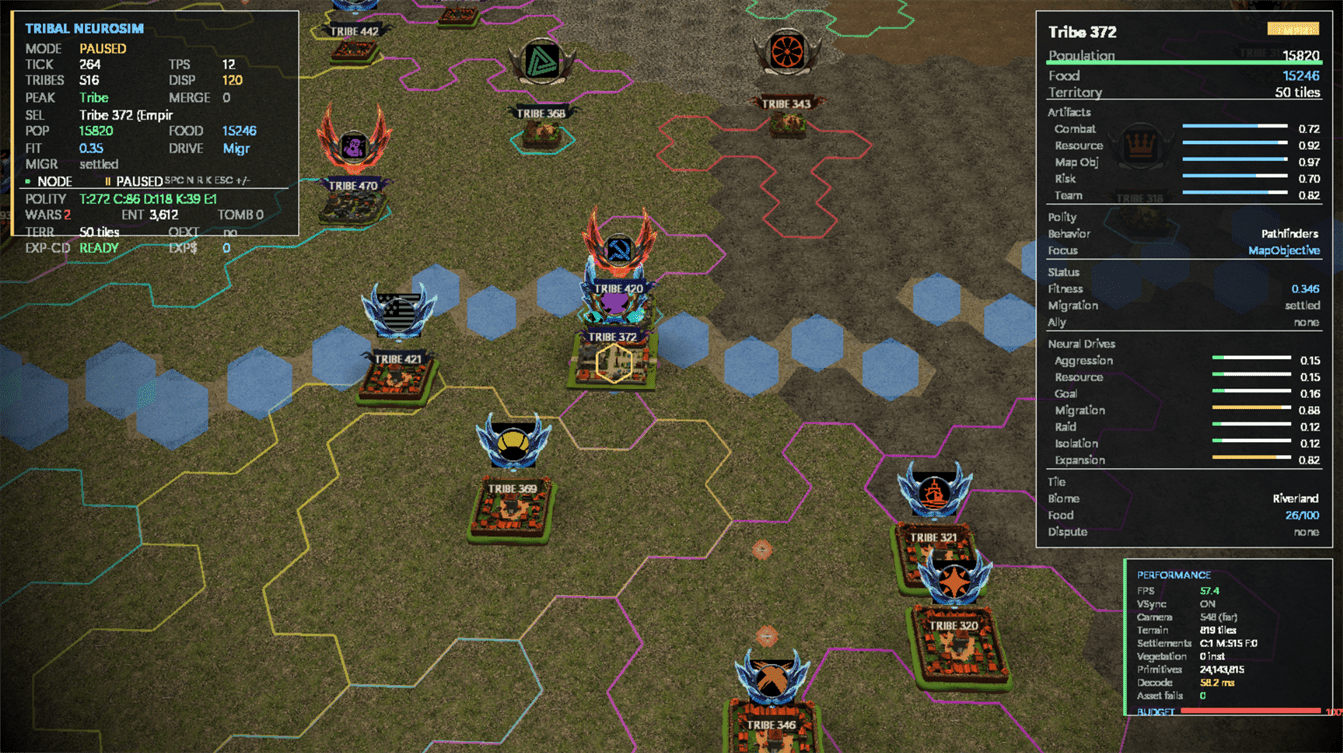
\includegraphics[width=0.9\textwidth]{assets/neurosim/run67fl7777-fl-s7777-tick264-firstempire.png}
\caption{Flexset, seed=7777, tick=264: az első Empire, Tribe 372, Pathfinders / MapObjective profillal.}
\label{fig:neurosim-run-fl7777-firstempire}
\end{figure}

\begin{figure}[h]
\centering
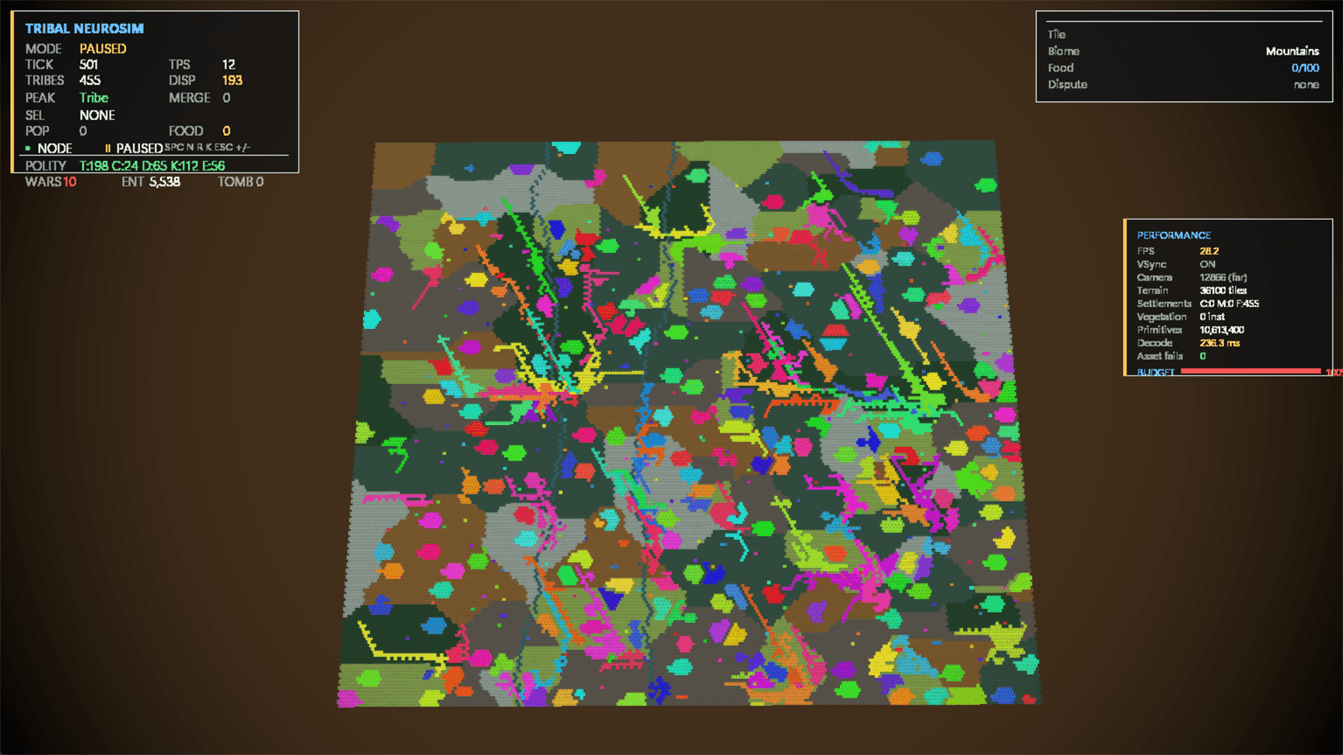
\includegraphics[width=0.9\textwidth]{assets/neurosim/run67fl7777-fl-s7777-tick500.png}
\caption{Flexset, seed=7777, tick=500: középső konszolidációs állapot, még sok kis- és középszintű entitással.}
\label{fig:neurosim-run-fl7777-tick500}
\end{figure}

\begin{figure}[h]
\centering
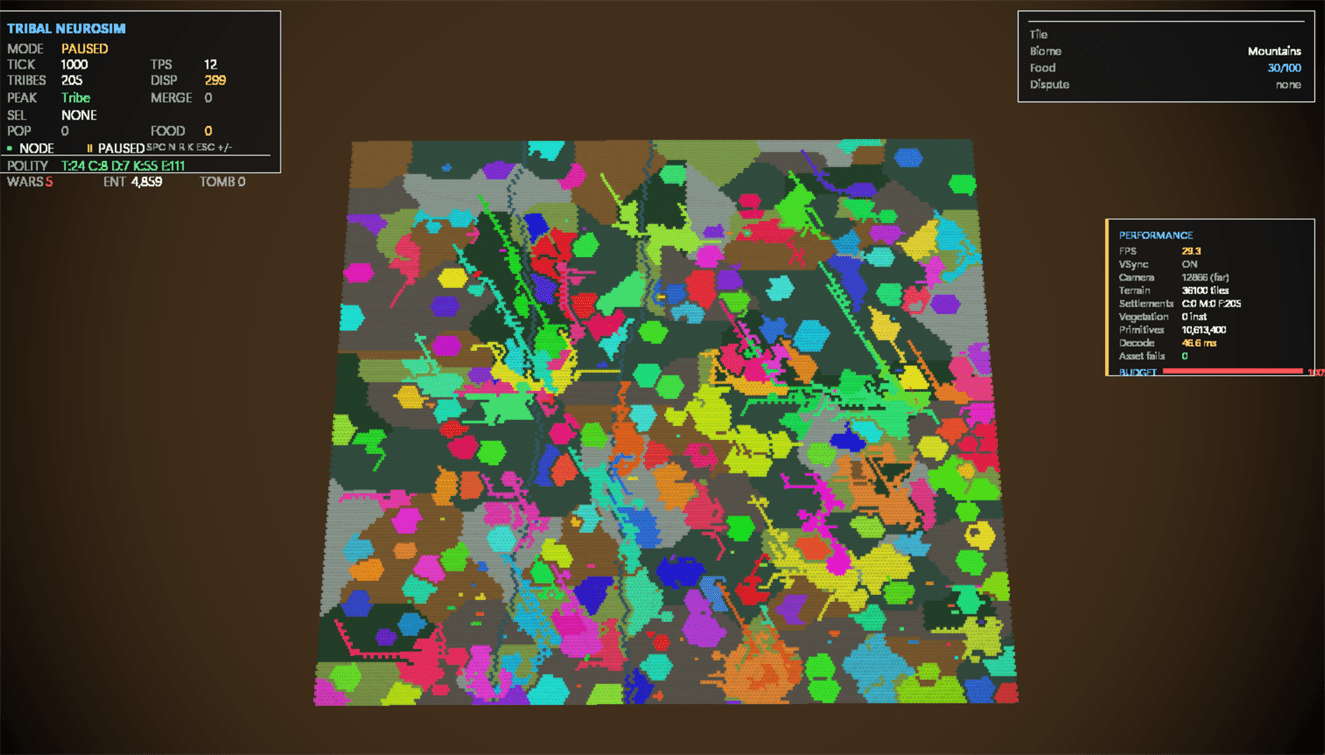
\includegraphics[width=0.9\textwidth]{assets/neurosim/run67fl7777-fl-s7777-tick1000.png}
\caption{Flexset, seed=7777, tick=1000: 205 túlélő; az Empire-korszak érdemben megkezdődött.}
\label{fig:neurosim-run-fl7777-tick1000}
\end{figure}

\begin{figure}[h]
\centering
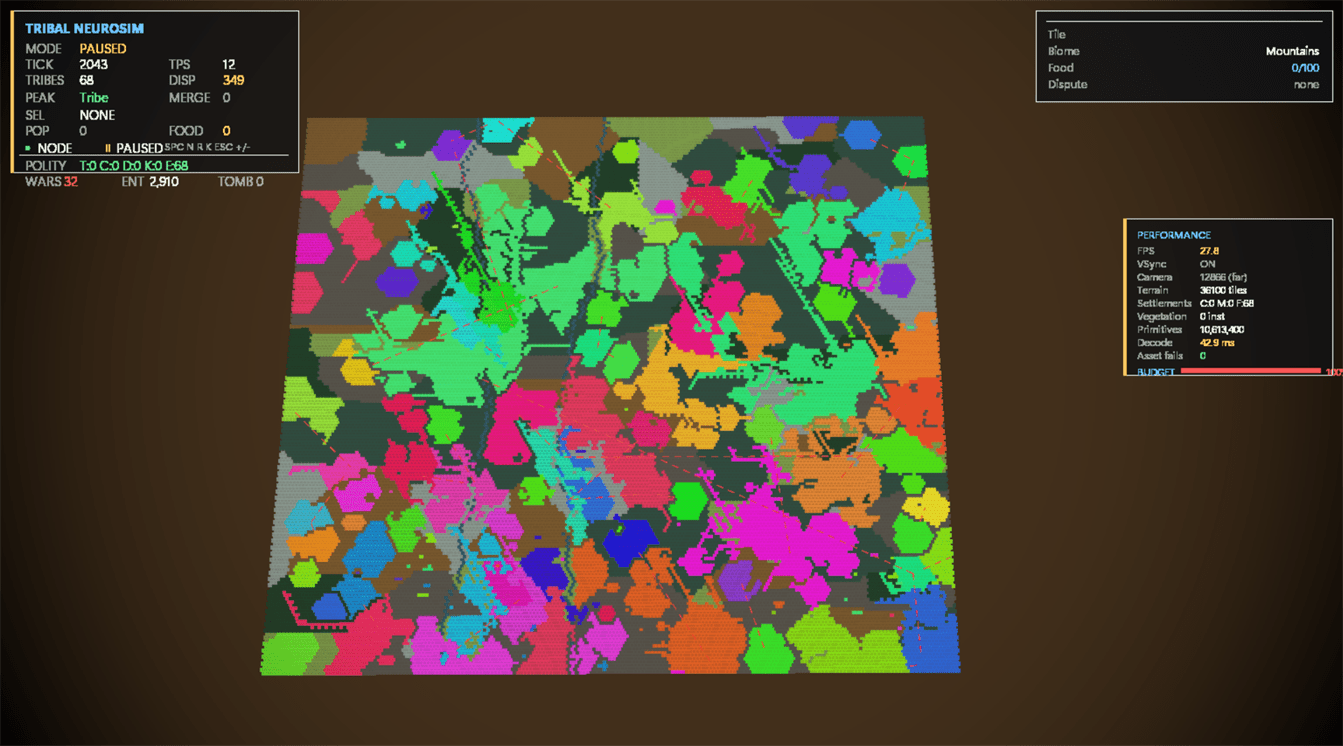
\includegraphics[width=0.9\textwidth]{assets/neurosim/run67fl7777-fl-s7777-tick2043-totalwar.png}
\caption{Flexset, seed=7777, tick=2043: a tick=2040-es Totális Háború utáni állapot, 68 túlélővel és 32 aktív háborúval.}
\label{fig:neurosim-run-fl7777-totalwar}
\end{figure}

\begin{figure}[h]
\centering
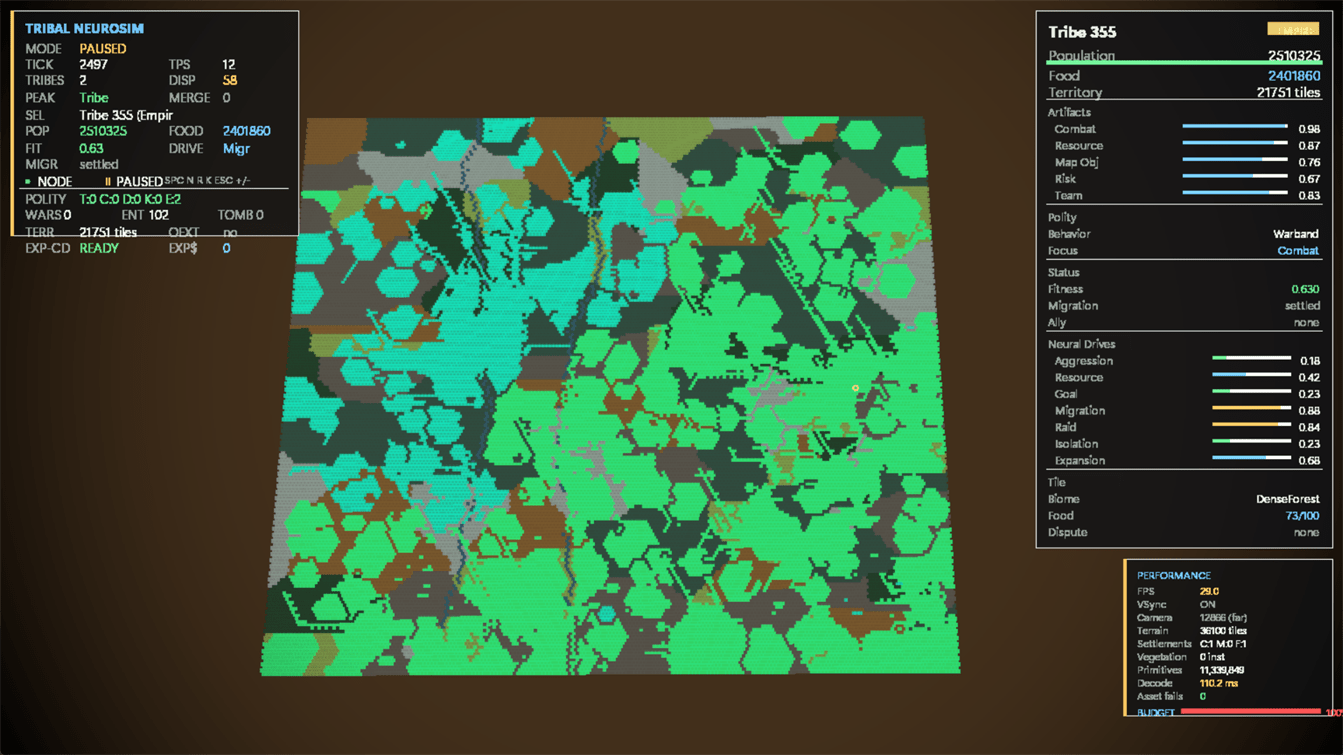
\includegraphics[width=0.9\textwidth]{assets/neurosim/run67fl7777-fl-s7777-tick2497-last2A.png}
\caption{Flexset, seed=7777, tick=2497: végső két szereplő, Tribe 355 profilja.}
\label{fig:neurosim-run-fl7777-last2a}
\end{figure}

\begin{figure}[h]
\centering
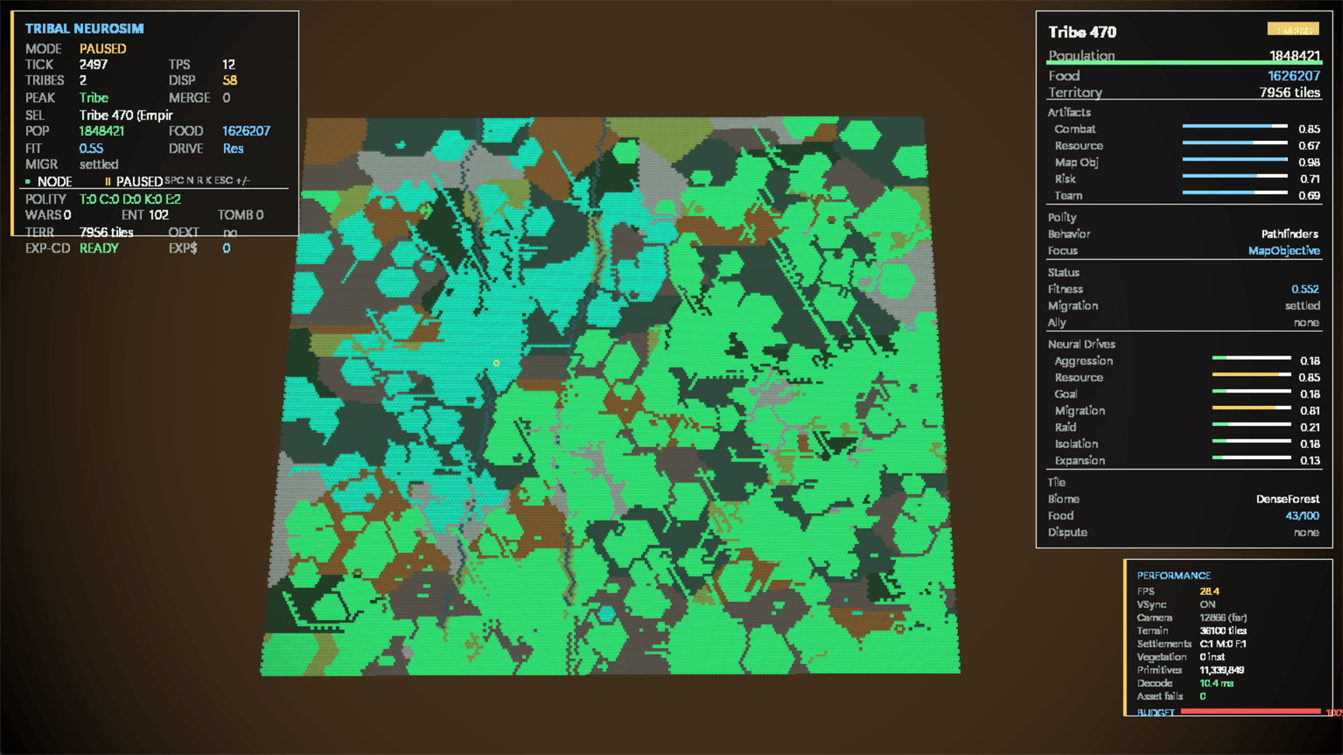
\includegraphics[width=0.9\textwidth]{assets/neurosim/run67fl7777-fl-s7777-tick2497-last2B.png}
\caption{Flexset, seed=7777, tick=2497: végső két szereplő, Tribe 470 profilja.}
\label{fig:neurosim-run-fl7777-last2b}
\end{figure}

\begin{figure}[h]
\centering
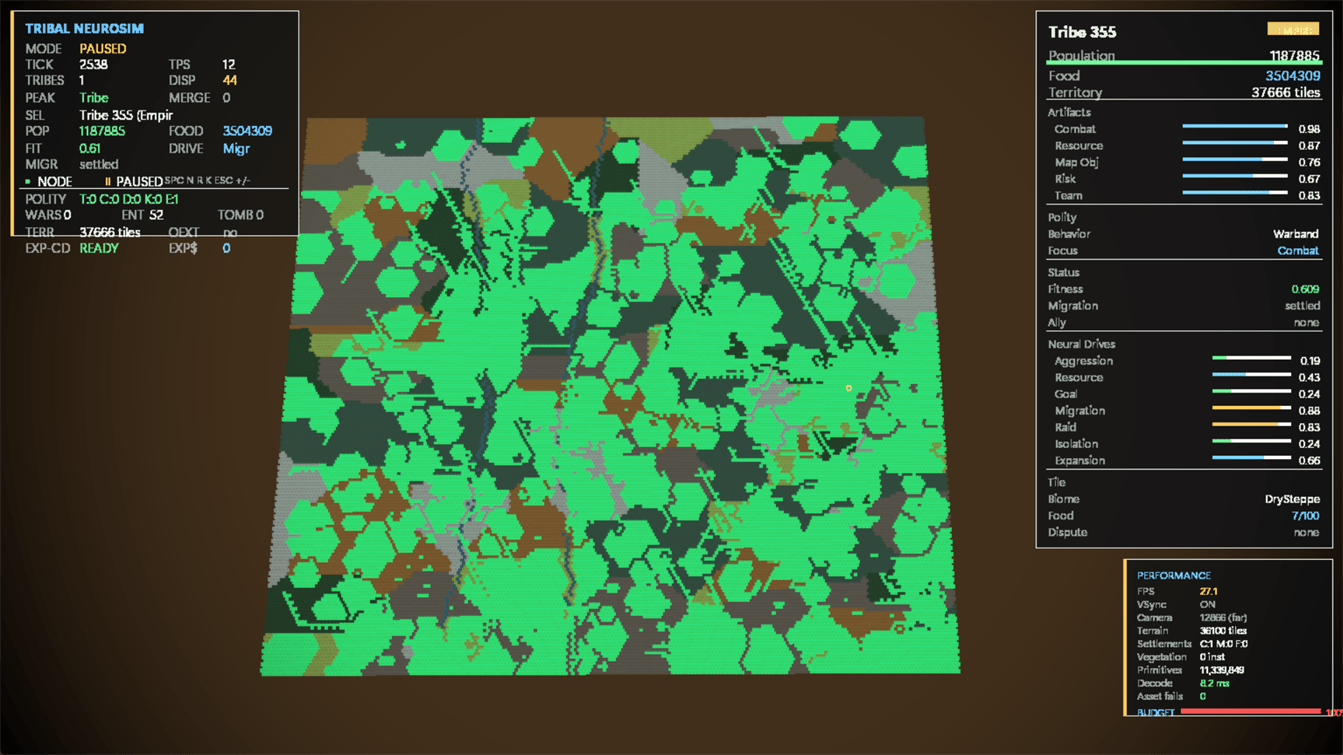
\includegraphics[width=0.9\textwidth]{assets/neurosim/run67fl7777-fl-s7777-tick2538-last.png}
\caption{Flexset, seed=7777, tick=2538: Tribe 355 győzelme, 37\,666 tile-os végső területtel.}
\label{fig:neurosim-run-fl7777-last}
\end{figure}

\subsection*{Flexset, seed=42}

\begin{table}[h]
\centering
\caption{Flexset seed=42 futtatás összefoglalója}
\label{tab:neurosim-run-fl42-summary}
\begin{tabular}{ll}
\hline
\textbf{Mező} & \textbf{Érték} \\
\hline
Adatkészlet & flexset (EUNE Master+ Flex Queue) \\
Seed & 42 \\
Indítótörzsek & 599 \\
Térkép & $\approx$36\,100 tile \\
Végső tick & 2487 \\
Győztes & Tribe 596 \\
Behavior / fókusz & Empire / Warband / Combat \\
Agresszió & 0,13 \\
Migráció & 0,87 \\
Kulcsesemény & Tick=2400 trilaterális háború Tribe 557 ellen \\
\hline
\end{tabular}
\end{table}

A flexset seed=42 futtatás ugyanazzal a 599 törzses Flex Queue inicializációs nagyságrenddel és $\approx$36\,100 tile-os térképpel indult, mint a seed=7777 változat, de a végjáték szerkezete eltért. A győztes Tribe 596 lett, szintén Empire / Warband / Combat profillal, 0,13-as agresszióval, 0,87-es migrációval és 0,96-os A\_combat értékkel. A két flexset futtatás közös tanulsága ezért erős: eltérő seed mellett is alacsony agressziójú, magas migrációjú, harci fókuszú Warband nyert.

A korai szakasz tick=287-nél hozta az első Empire-t. Tribe 220 Council / Team viselkedésű entitásként jelent meg, 15\,737 populációval, 68 tile-lal és 0,38-as fitnesszel. Ez különösen figyelemre méltó, mert a későbbi flexset győztesek Warband / Combat profilok voltak; az első fejlett polity itt kooperatív Council típus volt, nem a végül győztes archetípus előképe. Tick=500-nál Tribe 244 Warband / Combat entitásként 41\,042 populációt és 89 tile-t tartott, miközben 443 törzs még életben volt.

A középső szakaszban a seed=42 futtatás lassabban lépett át a teljes Empire-korszakba, mint a seed=7777, de a tick=900 és tick=950 közötti 64 kiesés itt is mass extinction burstként értelmezhető. Tick=1000-nél 234 túlélő volt, ebből 117 Empire. Tribe 596 ebben a fázisban nem domináns térképi szereplőként, hanem kitartó védőként építette fel harci értékét: a napló szerint Tribe 520 tick=300 körül, Tribe 521 tick=823-nál, majd Tribe 571 tick=939-nél támadta, és mindegyik támadó vereséget szenvedett.

A tömeges háborús fázis tick=1860-nál indult: 72 opportunity war deklaráció történt egyetlen tick alatt, ami nagyobb abszolút burst volt, mint a seed=7777 64 deklarációs Totális Háborúja. Tick=1872-nél 67 túlélő és 26 aktív háború látszott; 63 entitás már Empire-szintű volt. A 23.4.~alszekció konfliktusos struktúrái közül ez a futtatás előbb a tömeges opportunista kaszkádot, majd később a többfrontos, trilaterális nyomást mutatja be.

A döntő esemény tick=2400-nál következett be. Ekkor Tribe 90 és Tribe 596 egymástól függetlenül, ugyanabban a tickben támadta meg a domináns Tribe 557-et, amely a tick=2352-es Tribe 435 elleni győzelme után körülbelül 23\,149 tile-ra nőtt. A naplózott deklarációk szerint Tribe 90 agressziója 0,84, Tribe 596 agressziója 0,14 volt; vagyis ugyanaz a célpont két nagyon eltérő viselkedési profilból vált támadhatóvá. Tick=2417-nél a háromszereplős állapot még fennállt, majd tick=2424-nél Tribe 596 legyőzte Tribe 557-et, felszívta annak területét, és több mint 28\,000 tile-ra nőtt.

A végső párharc Tribe 90 és Tribe 596 között zajlott. Tick=2486-nál Tribe 90 Pathfinders / MapObjective profilként 11\,207 tile-on, 19\,366 populációval és 0,84-es agresszióval állt, míg Tribe 596 Warband / Combat profilként 28\,162 tile-t, 233\,960 populációt és 0,13-as agressziót tartott. Tribe 90 map-objective és risk értékei magasabbak voltak, de a trilaterális háborúban elvesztette populációs tartalékát. Tick=2487-nél Tribe 596 legyőzte Tribe 90-et, 329\,859 populációval, 2\,738\,854 food tartalékkal és 39\,369 tile-os végső területtel zárva a futtatást.

\begin{figure}[h]
\centering
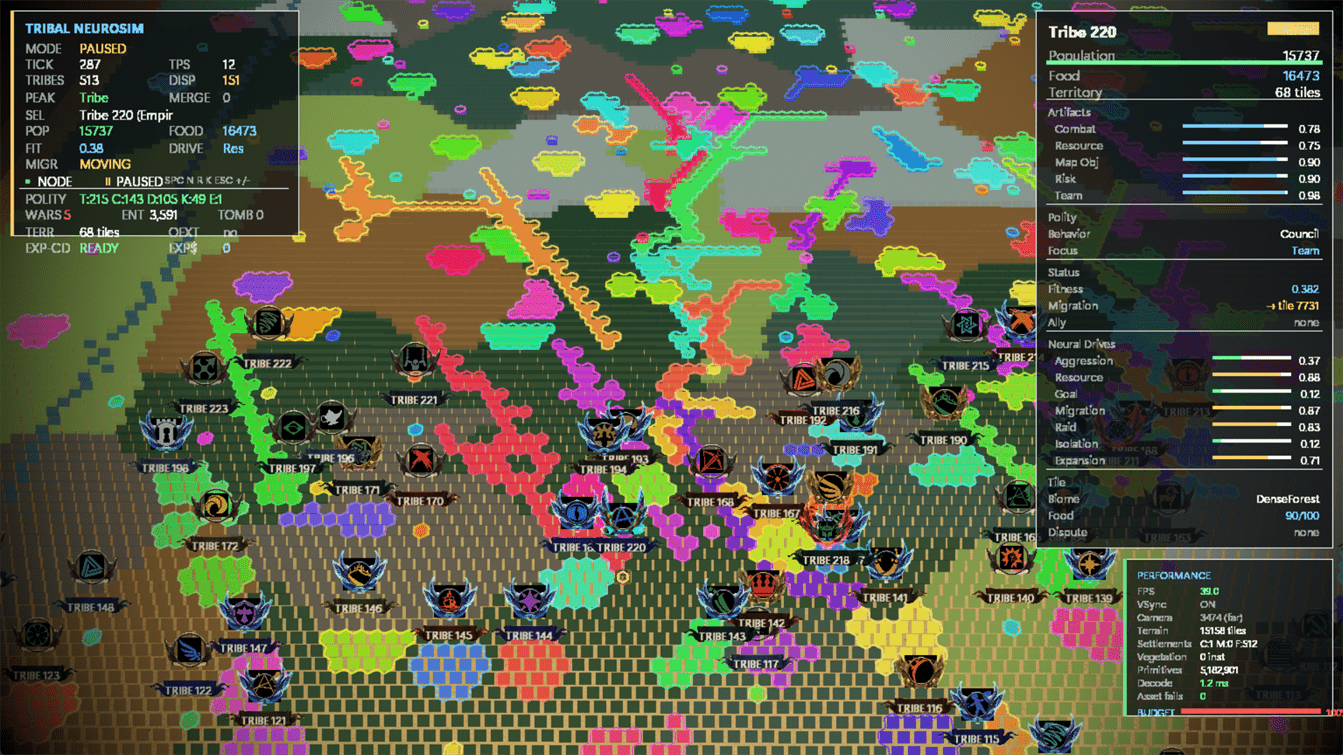
\includegraphics[width=0.9\textwidth]{assets/neurosim/run67fl42-fl-s42-tick287-firstempire.png}
\caption{Flexset, seed=42, tick=287: az első Empire, Tribe 220, Council / Team profillal.}
\label{fig:neurosim-run-fl42-firstempire}
\end{figure}

\begin{figure}[h]
\centering
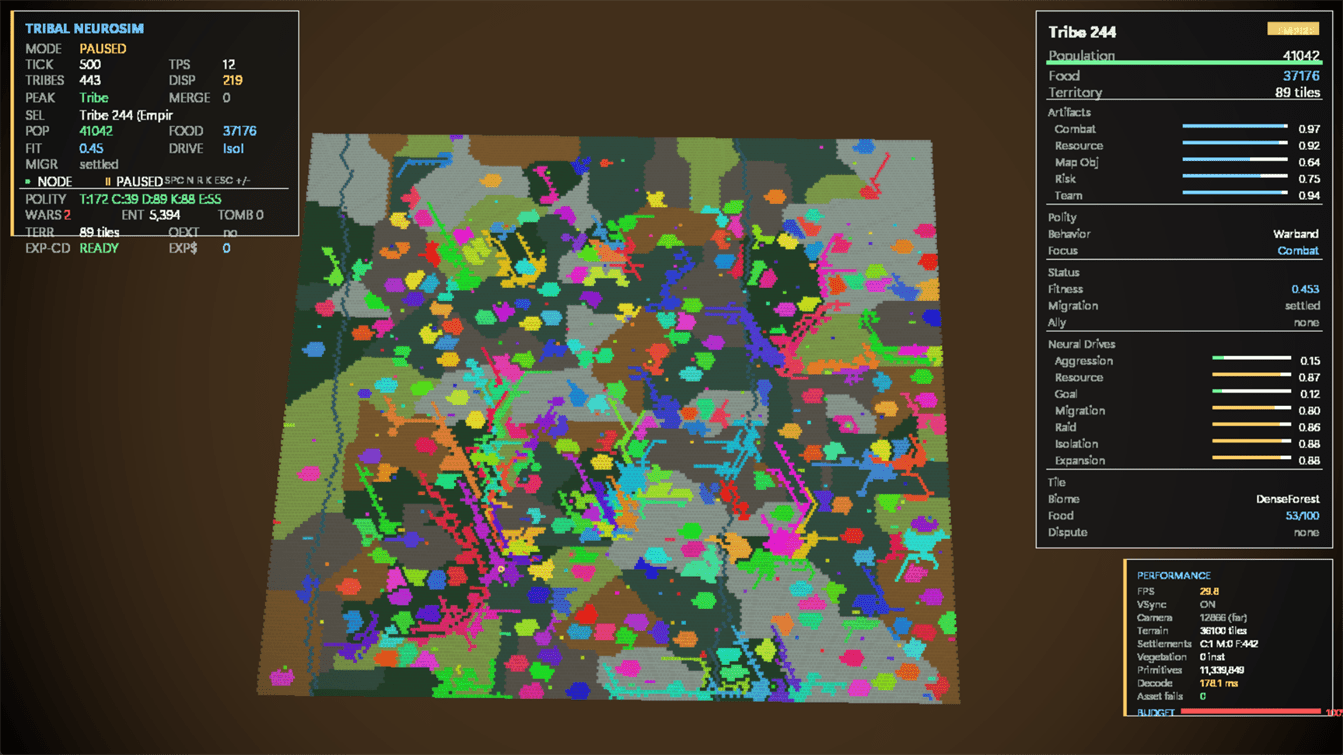
\includegraphics[width=0.9\textwidth]{assets/neurosim/run67fl42-fl-s42-tick500.png}
\caption{Flexset, seed=42, tick=500: középső konszolidáció, Tribe 244 kiemelt Warband / Combat profillal.}
\label{fig:neurosim-run-fl42-tick500}
\end{figure}

\begin{figure}[h]
\centering
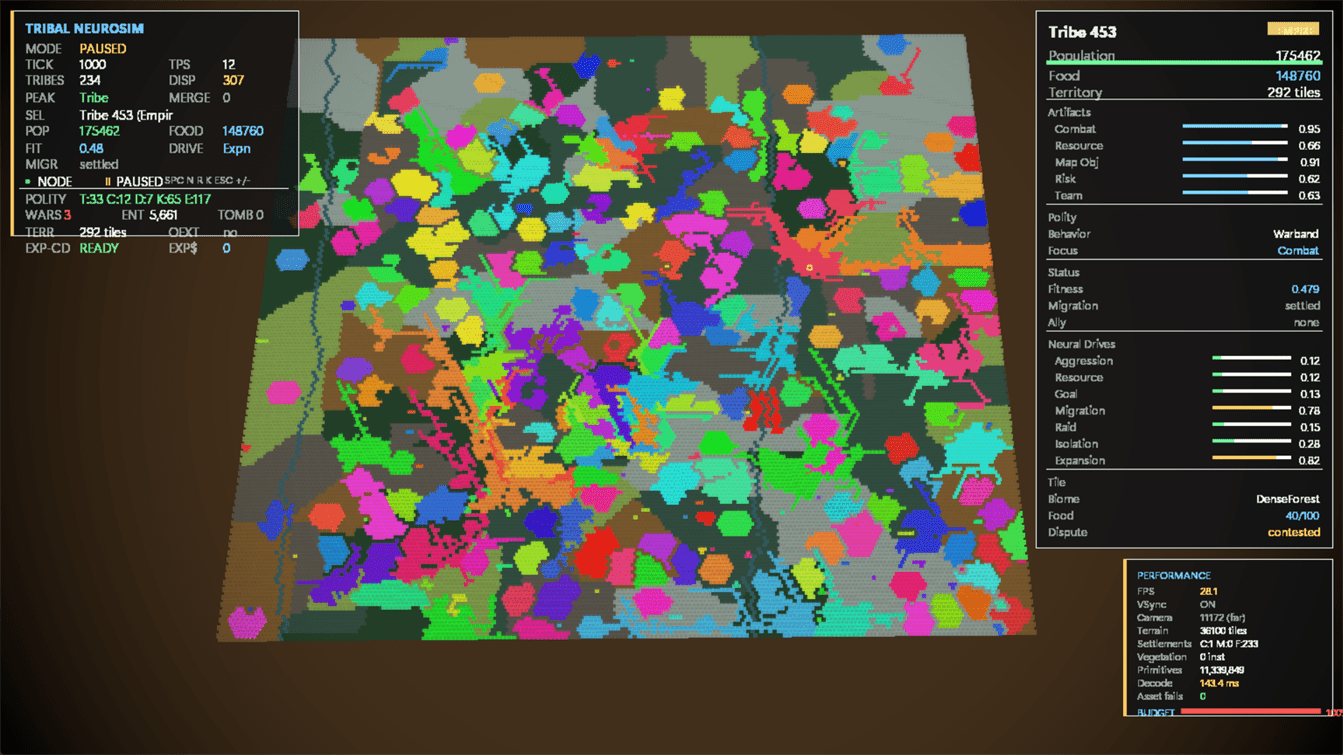
\includegraphics[width=0.9\textwidth]{assets/neurosim/run67fl42-fl-s42-tick1000.png}
\caption{Flexset, seed=42, tick=1000: Empire-korszak, 234 túlélővel.}
\label{fig:neurosim-run-fl42-tick1000}
\end{figure}

\begin{figure}[h]
\centering
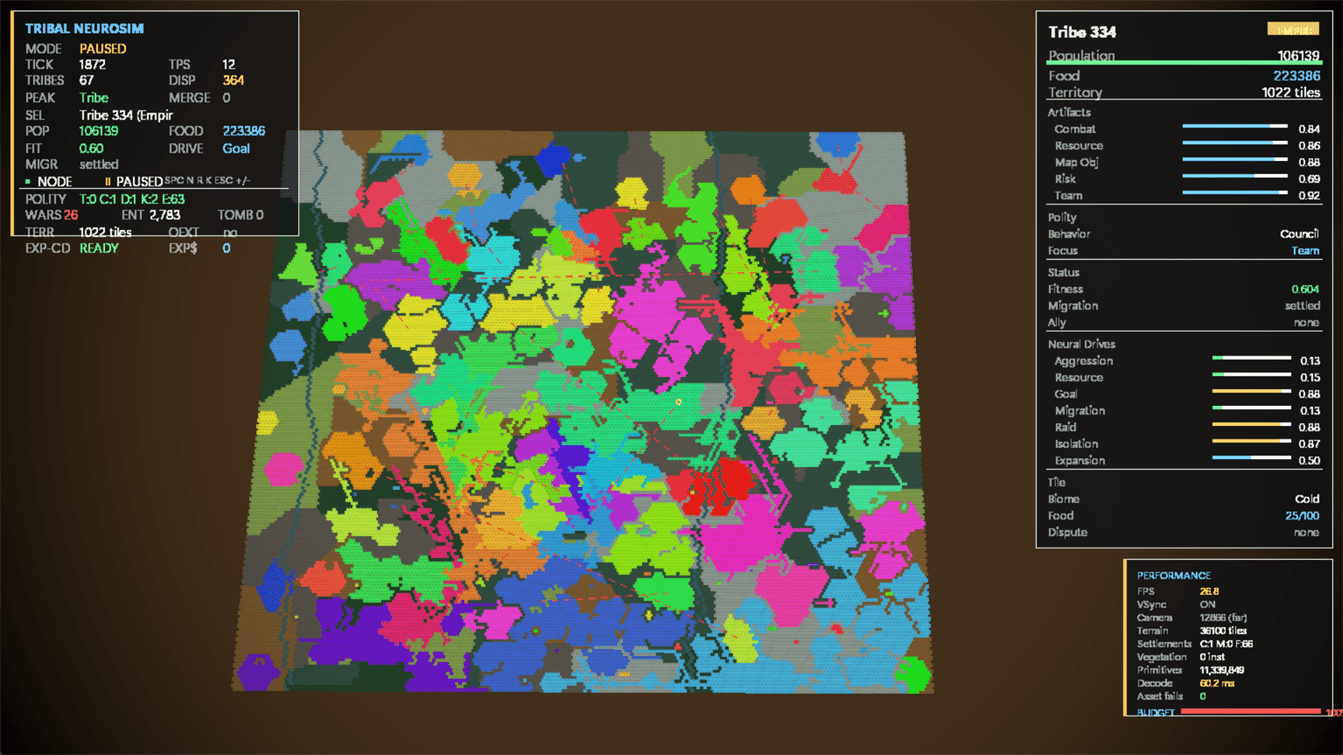
\includegraphics[width=0.9\textwidth]{assets/neurosim/run67fl42-fl-s42-tick1872-totalwar.png}
\caption{Flexset, seed=42, tick=1872: a tick=1860-as, 72 deklarációs Total War utáni állapot.}
\label{fig:neurosim-run-fl42-totalwar}
\end{figure}

\begin{figure}[h]
\centering
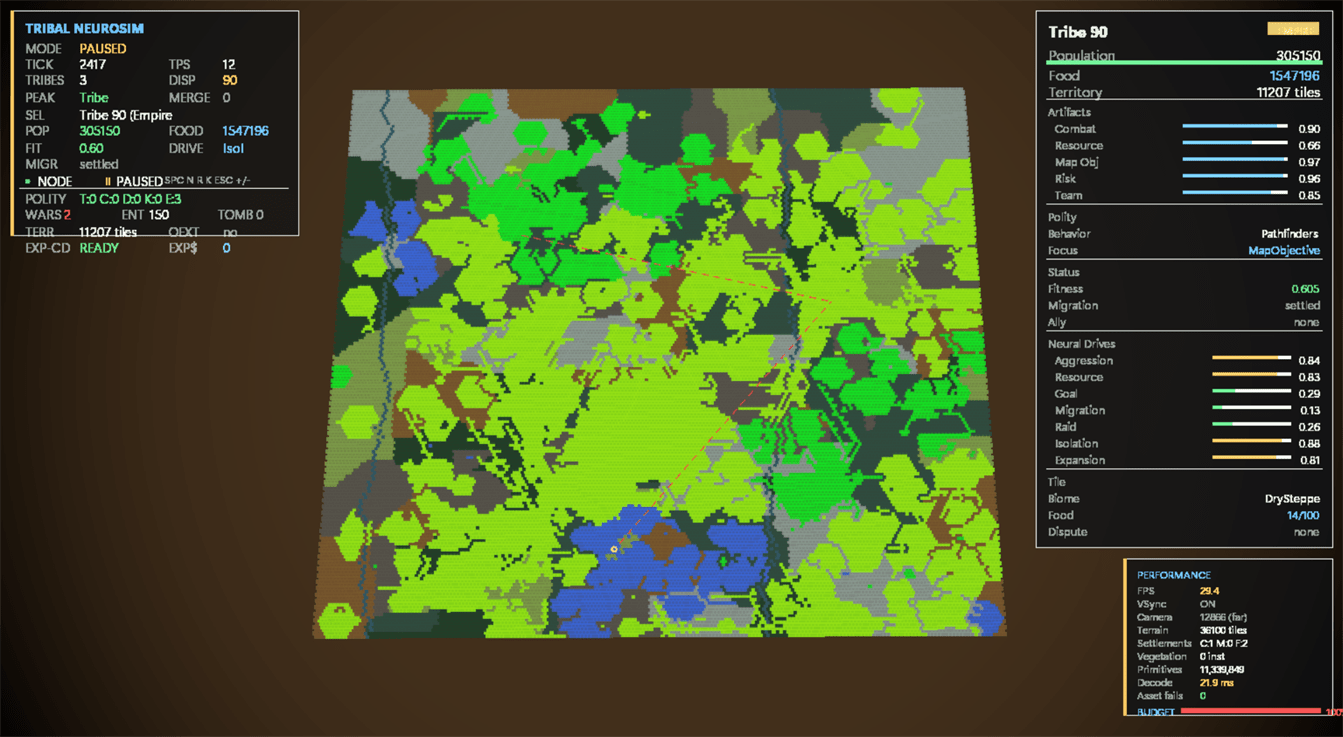
\includegraphics[width=0.9\textwidth]{assets/neurosim/run67fl42-fl-s42-tick2417-trilateralwar.png}
\caption{Flexset, seed=42, tick=2417: trilaterális háború Tribe 90, Tribe 596 és a domináns Tribe 557 között.}
\label{fig:neurosim-run-fl42-trilateralwar}
\end{figure}

\begin{figure}[h]
\centering
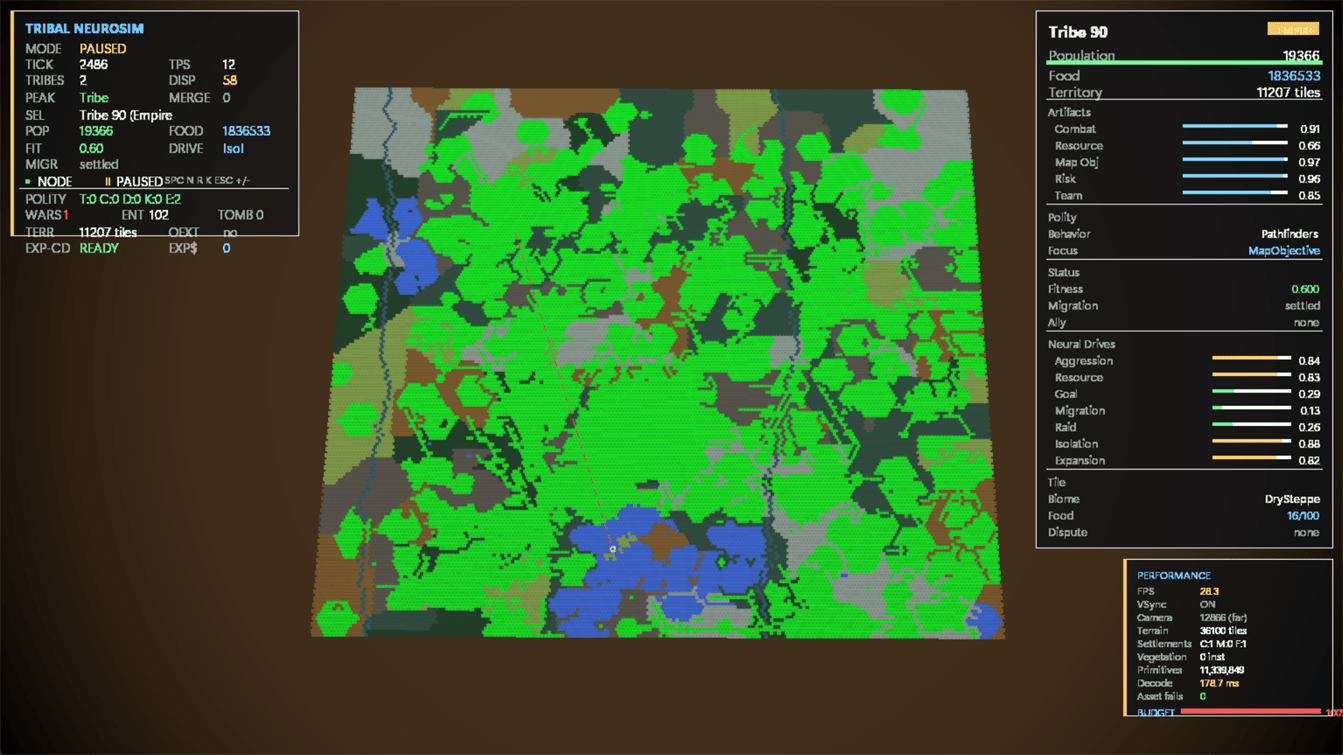
\includegraphics[width=0.9\textwidth]{assets/neurosim/run67fl42-fl-s42-tick2486-last2A.png}
\caption{Flexset, seed=42, tick=2486: végső két szereplő, Tribe 90 profilja.}
\label{fig:neurosim-run-fl42-last2a}
\end{figure}

\begin{figure}[h]
\centering
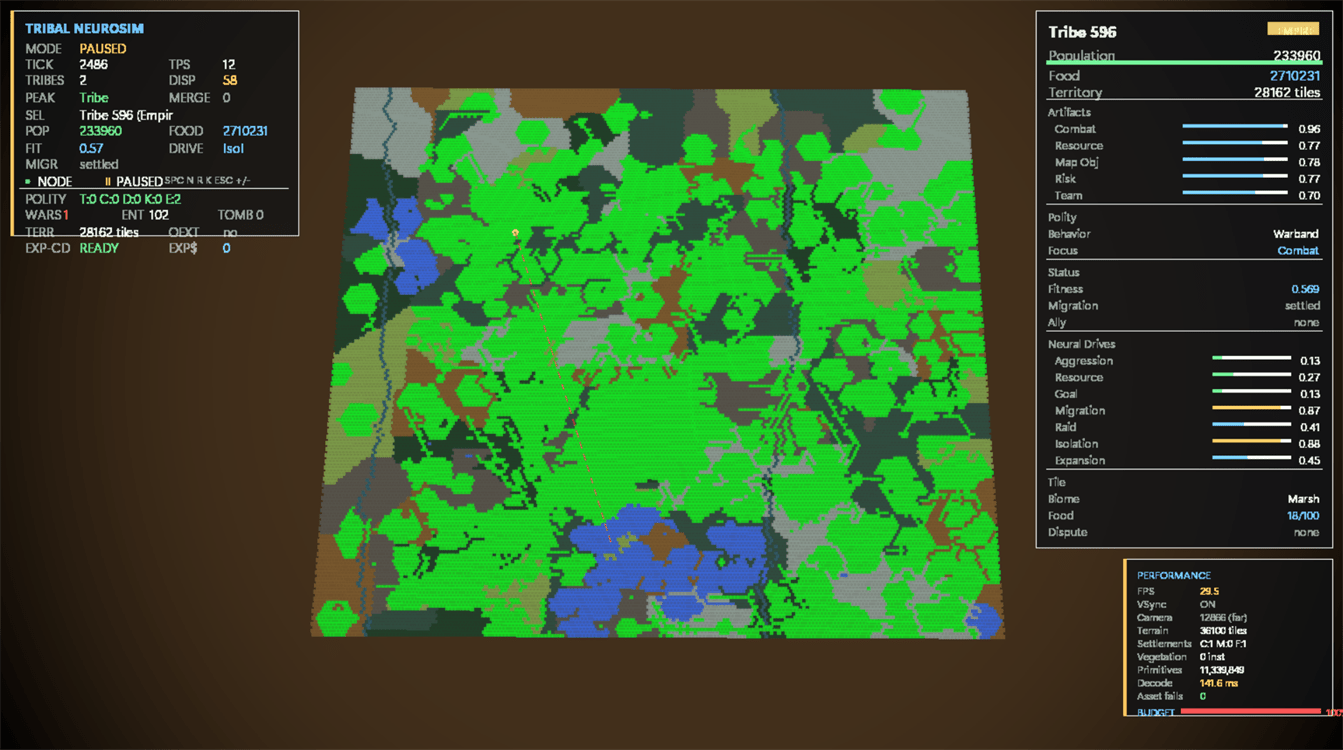
\includegraphics[width=0.9\textwidth]{assets/neurosim/run67fl42-fl-s42-tick2486-last2B.png}
\caption{Flexset, seed=42, tick=2486: végső két szereplő, Tribe 596 profilja.}
\label{fig:neurosim-run-fl42-last2b}
\end{figure}

\begin{figure}[h]
\centering
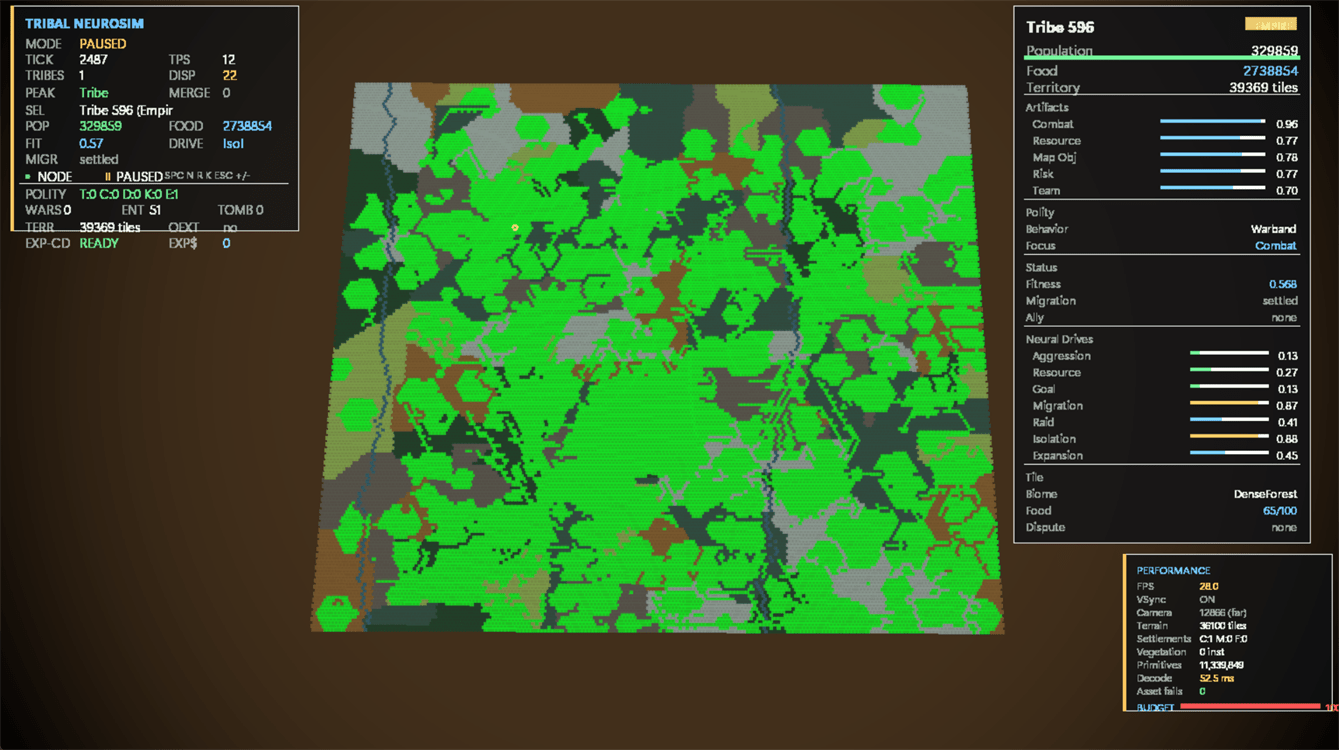
\includegraphics[width=0.9\textwidth]{assets/neurosim/run67fl42-fl-s42-tick2487-last.png}
\caption{Flexset, seed=42, tick=2487: Tribe 596 győzelme, 39\,369 tile-os végső területtel.}
\label{fig:neurosim-run-fl42-last}
\end{figure}

\subsection*{SoloQ, seed=42}

\begin{table}[h]
\centering
\caption{SoloQ seed=42 futtatás összefoglalója}
\label{tab:neurosim-run-sq42-summary}
\begin{tabular}{ll}
\hline
\textbf{Mező} & \textbf{Érték} \\
\hline
Adatkészlet & soloq (EUNE Master+ Solo Queue) \\
Seed & 42 \\
Indítótörzsek & 140 \\
Térkép & végső győztes terület: 6\,356 tile \\
Végső tick & 2046, a leggyorsabb futtatás \\
Győztes & Tribe 89 \\
Behavior / fókusz & Empire / Vanguard / Risk \\
Agresszió & 0,13 \\
Migráció / raid / izoláció & 0,16 / 0,14 / 0,88 \\
Kulcsesemény & Tick=1740 Total War; tick=1926--1935 védelmi sorozat \\
\hline
\end{tabular}
\end{table}

A SoloQ seed=42 futtatás 140 törzzsel és a végállapotban 6\,356 tile-os győztes területtel zárult tick=2046-nál, ezzel a négy futtatás közül a leggyorsabb volt. A győztes Tribe 89 Empire / Vanguard / Risk profilú entitás lett. Ez az archetípus élesen eltér a flexset győztesektől: itt nem Warband / Combat, hanem alacsony agressziójú, magas izolációjú és risk-fókuszú Vanguard nyert. A győztes képernyőképen 0,13-as aggression, 0,16-os migration, 0,14-es raid és 0,88-as isolation érték látható.

A nyitás paradox módon békésebb volt, mint a későbbi gyors végjáték sugallná. Tick=50-nél és tick=100-nál még egyetlen törzs sem halt meg; ez volt az egyetlen futtatás, ahol az első 100 tick nem hozott eliminációt. A háborúk tick=120 után gyorsultak fel, tick=150-nél már 135 túlélő és 7 aktív háború volt. Az első Empire tick=286-nál Tribe 88 volt: Council / Team viselkedésű, 5\,337 populációval, 97 tile-lal és 0,38-as fitnesszel. Ez korai kooperatív fejlettséget jelez, de nem győztes archetípust.

Tick=300 és tick=900 között a kis térkép gyorsan megtelt. Tick=500-nál 101 törzs élt, tick=1000-nél már csak 59, ebből 33 Empire. Tick=650 és tick=700 között az alive count 91-en stagnált, aktív háború nélkül; ez a kisebb térkép megfelelője annak a trench-stagnation jelenségnek, amely a SoloQ seed=7777 futtatásban később, hosszabb ideig jelent meg. A diplomáciai szövet tick=1450--1500 körül már alig létezett: az alliance count 4 körüli padlóra esett.

A döntő fordulat tick=1740-nél történt. A Total War esemény 16 egyidejű opportunity war deklarációt indított, és 23 túlélőből tick=1750-re 14-et hagyott meg: 9 entitás esett ki egy burst alatt, ami 39\%-os mezőnyvesztést jelent. A 23.4.~alszekció konfliktustáblázatának terminológiájával ez arányában rendkívül intenzív tömeges opportunista kaszkád, még akkor is, ha abszolút deklarációszáma kisebb, mint a flexset futtatásoké.

Tribe 89 tick=1860 és tick=1983 között vált döntő szereplővé. Tick=1860-nál megtámadta és legyőzte Tribe 123-at, tick=1920-nál Tribe 32-t, majd tick=1926--1935 között három egymást követő védelmi háborút nyert: Tribe 132 tick=1926-nál, Tribe 36 tick=1935-nél és Tribe 130 szintén tick=1935-nél támadta, és mindhárom támadó meghalt a támadás közben. Ez a futtatás legfontosabb mikronarratívája: Tribe 89 nem agresszív expanzióval, hanem célzott raid-képességgel és védelmi túléléssel vált dominánssá.

Tick=1987-nél már csak Tribe 89 és Tribe 10 maradt. A különbség ekkor már nemcsak területi, hanem populációs is volt: Tribe 89 798\,224 populációt és 5\,865 tile-t tartott, míg Tribe 10 29\,045 populációra és 487 tile-ra szorult vissza. Tribe 10 magasabb A\_resource és magas goal drive értéket mutatott, de erőforrás- és térbeli mozgástere elfogyott. Tick=2040-nél még egy utolsó opportunity raid-et indított, majd tick=2046-nál Tribe 89 győzött. A végállapot: 929\,629 populáció, 1\,175\,612 food és 6\,356 tile.

\begin{figure}[h]
\centering
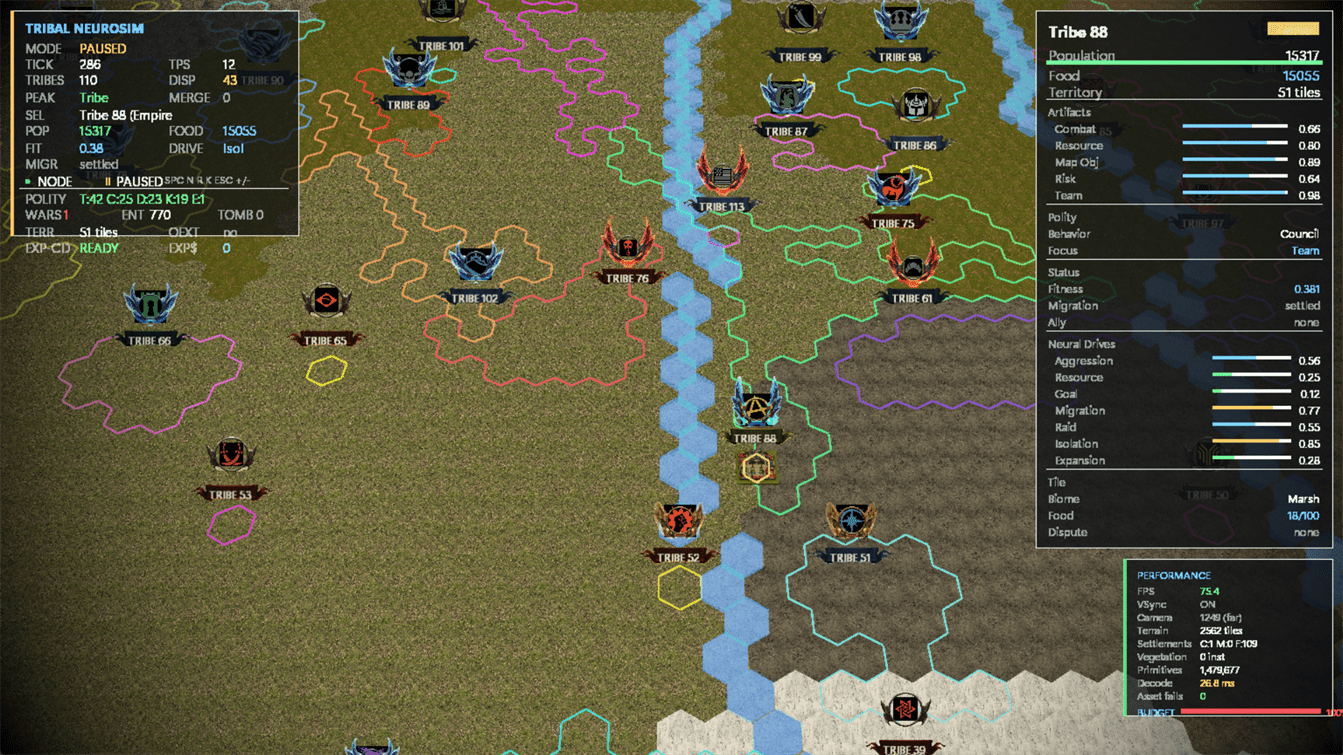
\includegraphics[width=0.9\textwidth]{assets/neurosim/run67sq42-sq-s42-tick286-firstempire.png}
\caption{SoloQ, seed=42, tick=286: az első Empire, Tribe 88, Council / Team profillal.}
\label{fig:neurosim-run-sq42-firstempire}
\end{figure}

\begin{figure}[h]
\centering
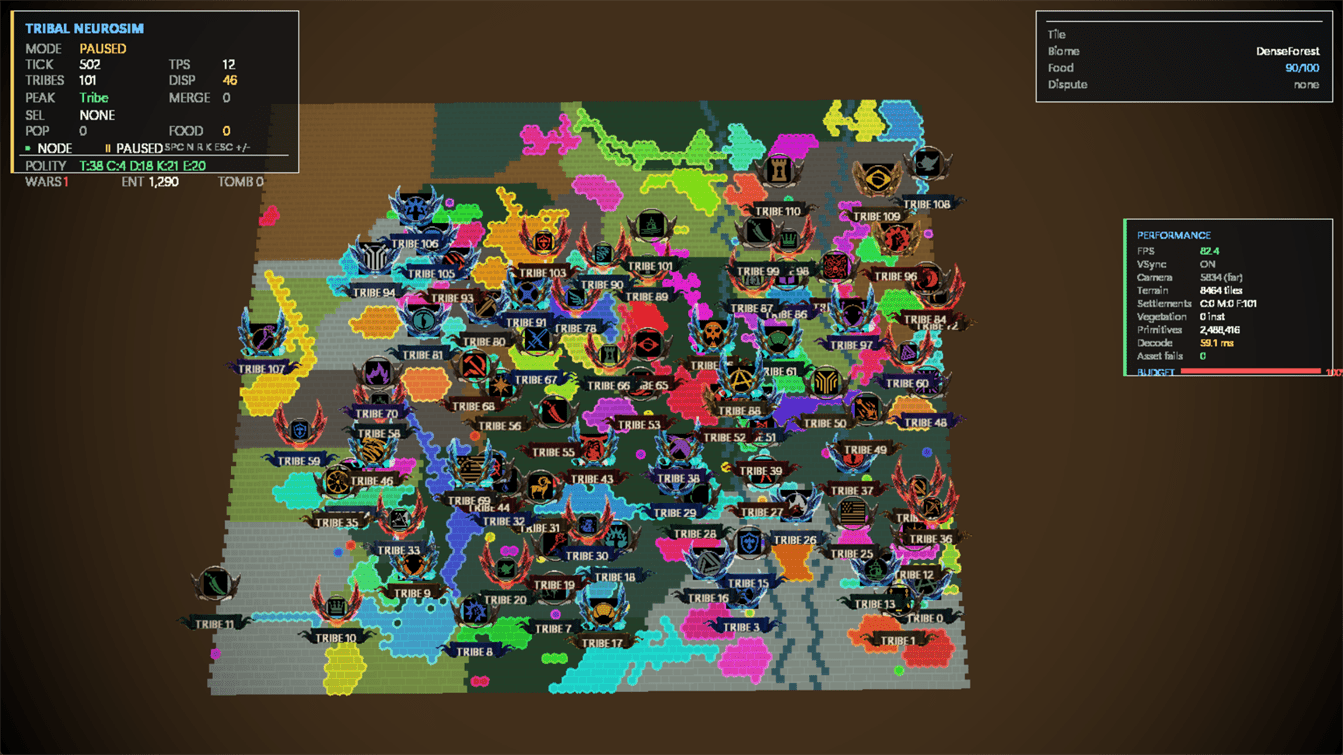
\includegraphics[width=0.9\textwidth]{assets/neurosim/run67sq42-sq-s42-tick500.png}
\caption{SoloQ, seed=42, tick=500: 101 túlélő a kis, sűrű térképen.}
\label{fig:neurosim-run-sq42-tick500}
\end{figure}

\begin{figure}[h]
\centering
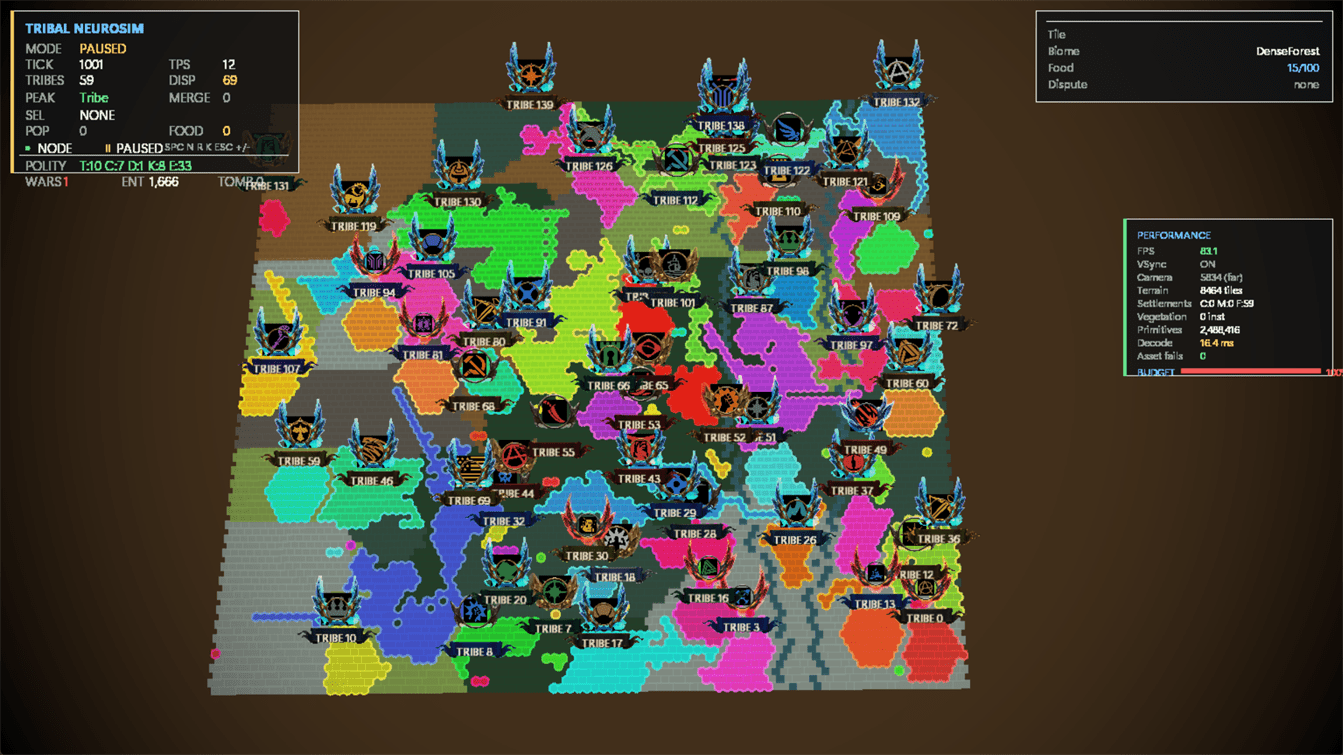
\includegraphics[width=0.9\textwidth]{assets/neurosim/run67sq42-sq-s42-tick1000.png}
\caption{SoloQ, seed=42, tick=1000: 59 túlélő, 33 Empire; a térkép nagy része már lefedett.}
\label{fig:neurosim-run-sq42-tick1000}
\end{figure}

\begin{figure}[h]
\centering
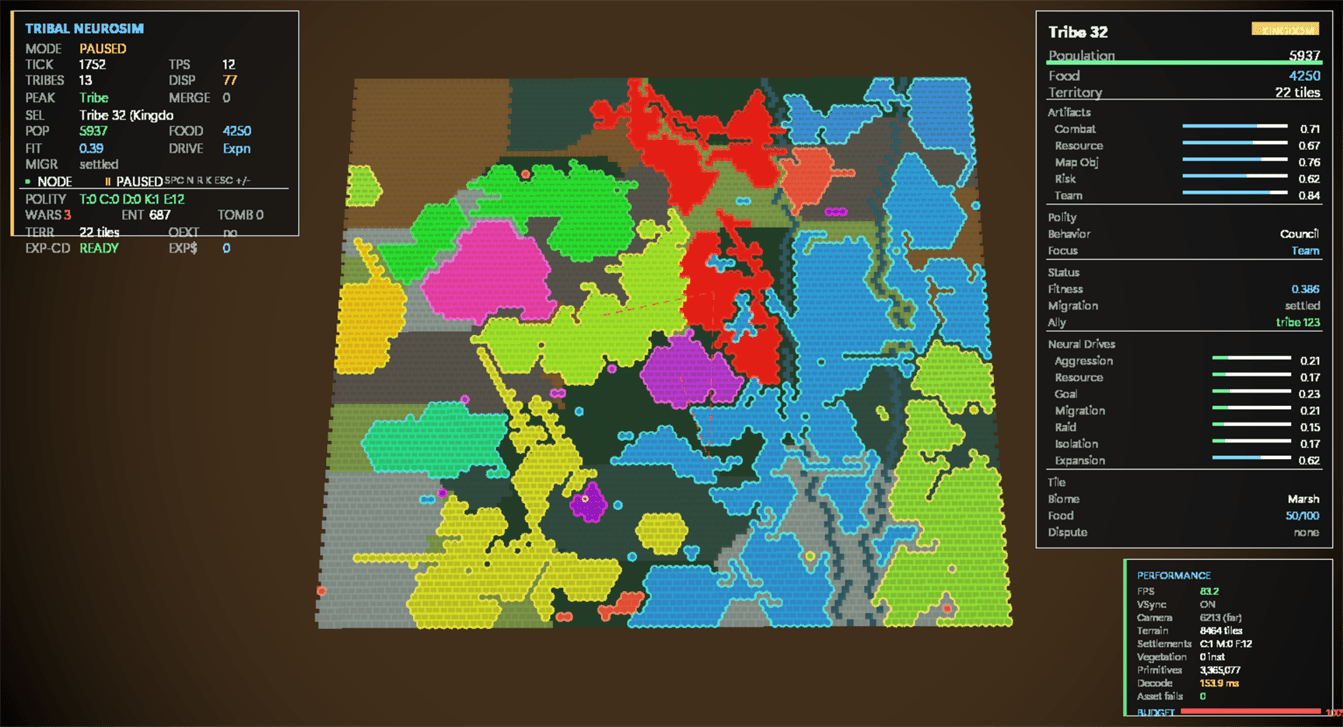
\includegraphics[width=0.9\textwidth]{assets/neurosim/run67sq42-sq-s42-tick1752-totalwar.png}
\caption{SoloQ, seed=42, tick=1752: a tick=1740-es Total War utáni állapot, 13 túlélővel és 5 aktív háborúval.}
\label{fig:neurosim-run-sq42-totalwar}
\end{figure}

\begin{figure}[h]
\centering
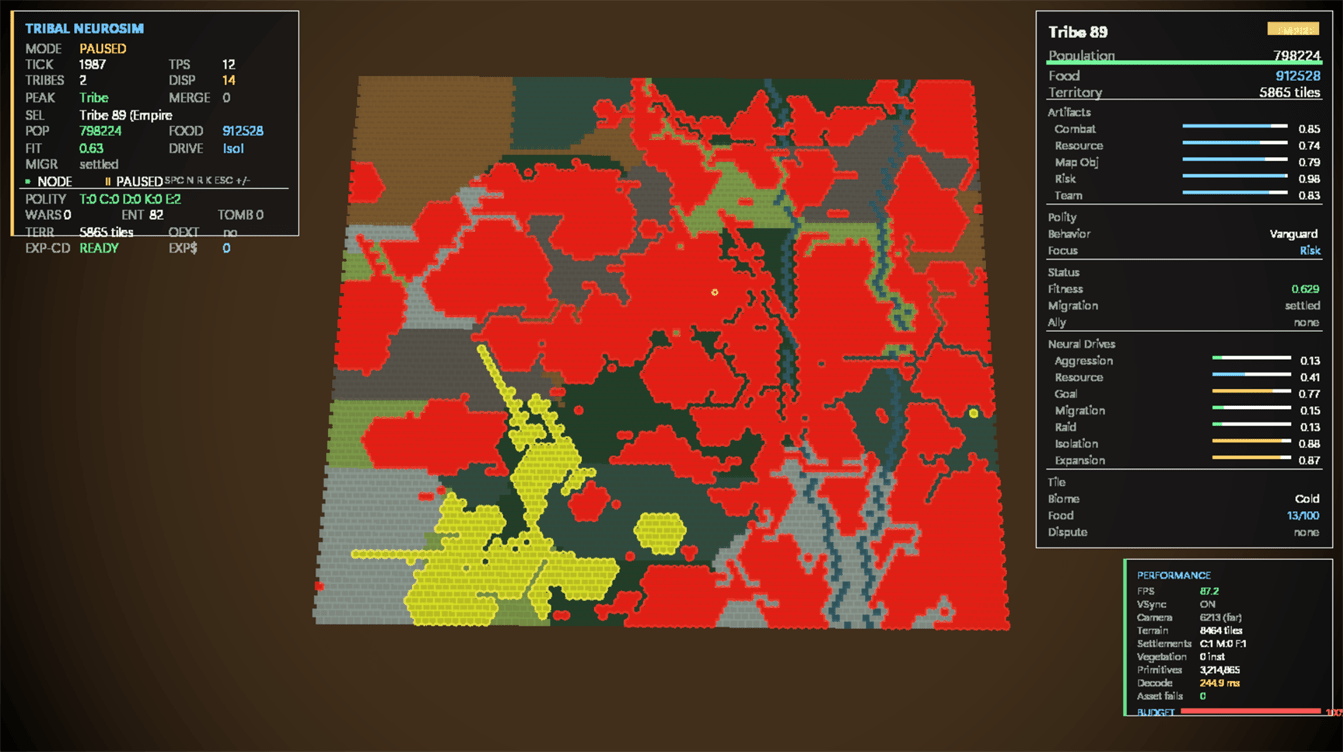
\includegraphics[width=0.9\textwidth]{assets/neurosim/run67sq42-sq-s42-tick1987-last2A.png}
\caption{SoloQ, seed=42, tick=1987: végső két szereplő, Tribe 89 domináns területi helyzetben.}
\label{fig:neurosim-run-sq42-last2a}
\end{figure}

\begin{figure}[h]
\centering
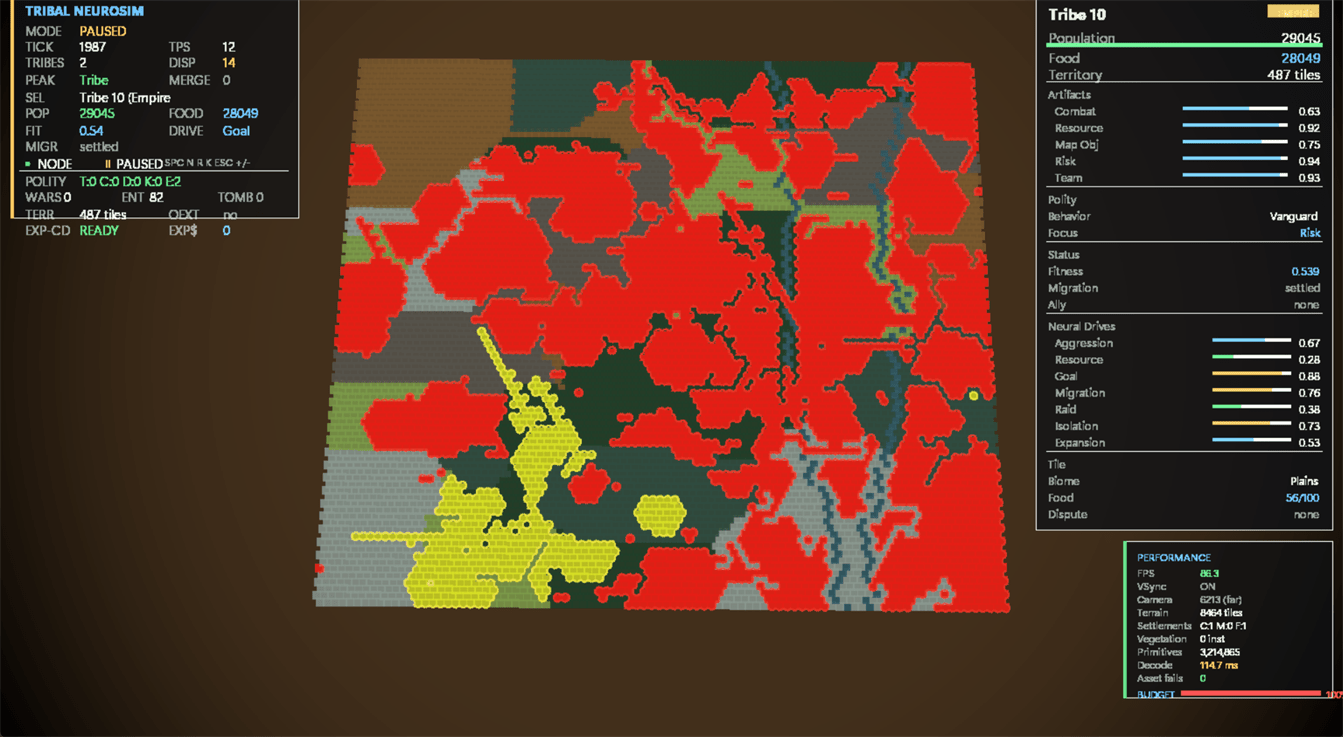
\includegraphics[width=0.9\textwidth]{assets/neurosim/run67sq42-sq-s42-tick1987-last2B.png}
\caption{SoloQ, seed=42, tick=1987: végső két szereplő, Tribe 10 sarokba szorított állapotban.}
\label{fig:neurosim-run-sq42-last2b}
\end{figure}

\begin{figure}[h]
\centering
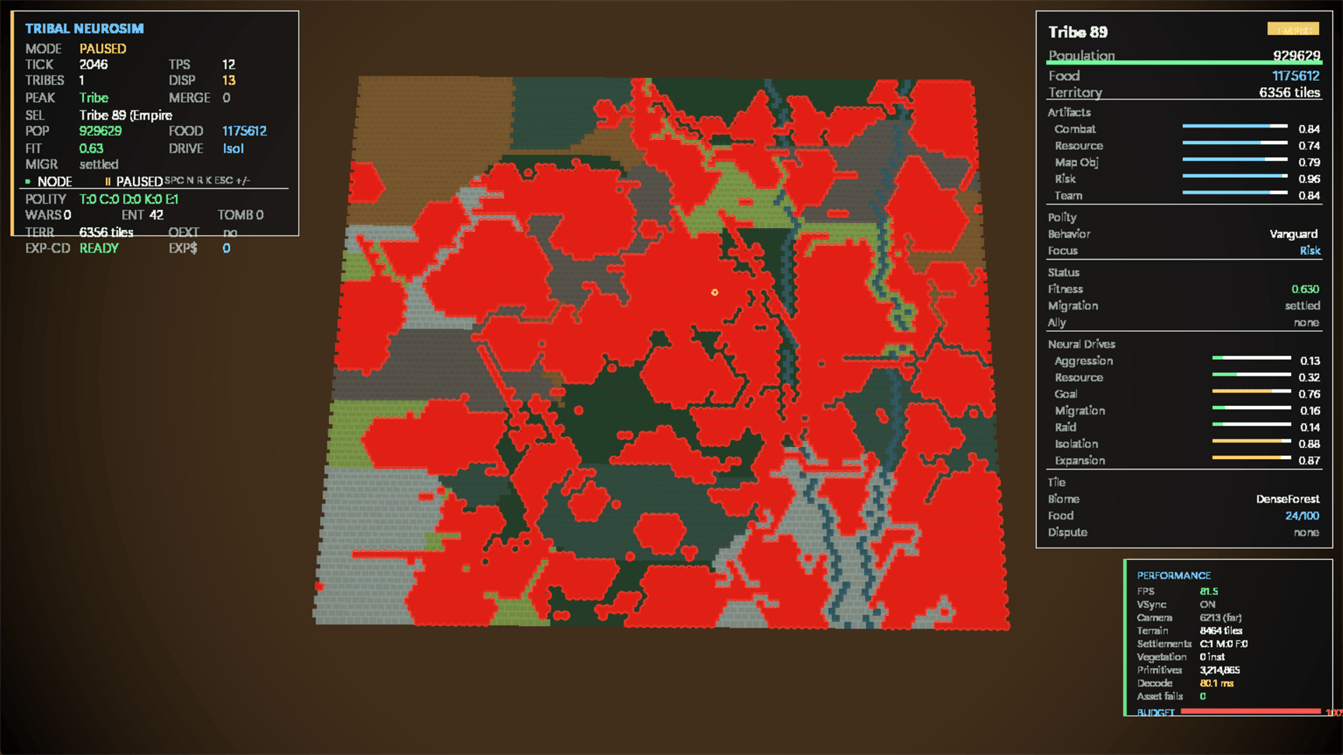
\includegraphics[width=0.9\textwidth]{assets/neurosim/run67sq42-sq-s42-tick2046-last.png}
\caption{SoloQ, seed=42, tick=2046: Tribe 89 győzelme, 6\,356 tile-os végső területtel.}
\label{fig:neurosim-run-sq42-last}
\end{figure}

\subsection*{SoloQ, seed=7777}

\begin{table}[h]
\centering
\caption{SoloQ seed=7777 futtatás összefoglalója}
\label{tab:neurosim-run-sq7777-summary}
\begin{tabular}{ll}
\hline
\textbf{Mező} & \textbf{Érték} \\
\hline
Adatkészlet & soloq (EUNE Master+ Solo Queue) \\
Seed & 7777 \\
Indítótörzsek & 140 \\
Térkép & végső győztes terület: 9\,748 tile \\
Végső tick & 2541 \\
Győztes & Tribe 70 \\
Behavior / fókusz & Empire / Supply / Resource \\
Agresszió & 0,88 \\
Migráció / izoláció / raid & 0,87 / 0,88 / 0,43 \\
Kulcsesemény & Tribe 99 középső dominanciája, majd tick=2340-es bukása \\
\hline
\end{tabular}
\end{table}

A SoloQ seed=7777 futtatás 140 törzzsel és tick=2541-es végállapottal zárult. A győztes Tribe 70 Empire / Supply / Resource profilú entitás volt, 0,88-as agresszióval, 0,87-es migrációval, 0,88-as isolation értékkel és 0,43-as raid drive-val a győztes képernyőkép alapján. Ez a negyedik futtatás teszi explicitté az adatkészlet-függő archetípus-különbséget: ugyanazzal a seed-del a flexset Warband / Combat győztest adott, míg a SoloQ Supply / Resource győztest, magas agressziós és resource komponenssel.

A korai szakasz nyugodtabb volt, mint a flexset megfelelője. Tick=50-nél mind a 140 törzs élt, tick=100-nál csak egy törzs esett ki. Az első Empire tick=300-nál jelent meg, a tick=301-es képen Tribe 19 látható Warband / Combat profillal, 10\,844 populációval, 47 tile-lal és 0,33-as fitnesszel. Ekkor 122 törzs volt életben, tehát az Empire-küszöb korai elérése itt sem jelentett végső dominanciát; Tribe 19 csak tick=2505-nél esett ki, vagyis polity-szint szerint a futtatás egyik leghosszabb túlélője maradt.

A középső szakasz főszereplője Tribe 99 volt. A log szerint már tick=147-nél legyőzte Tribe 100-at, majd hosszú sorozatban további győzelmeket aratott: Tribe 76 tick=387-nél, Tribe 61 tick=1239-nél, Tribe 101 tick=1392-nél, Tribe 92 tick=1692-nél, Tribe 85 tick=1935-nél és Tribe 124 tick=2091-nél esett ki ellene. A napló ezen kívül több védelmi győzelmet is rögzít Tribe 99 körül, ezért itt nem egyetlen csatáról, hanem tartós front-runner szerepről van szó. Ez a minta a SoloQ futtatások individualizáltabb, front-runner jellegű dinamikáját mutatja.

Tick=1000 és tick=2000 között a futtatás hosszú stagnációt produkált. Tick=1000-nél 61, tick=1500-nál 40, tick=1850-nél még mindig 32 törzs élt; tick=1550 és tick=1850 között az alive count alig mozdult. A térkép ekkorra nagyrészt felosztottá vált, a nagy Empire-ek pedig ritkábban találtak kedvező opportunista támadási ablakot. A flexset tömeges kaszkádjaihoz képest ez lassabb, egyéni háborúkra épülő konszolidáció.

A Totális Háború tick=2100-nál indult, 17 egyidejű opportunity war deklarációval. Tick=2110-nél 18 túlélő, 7 aktív háború és kizárólag Empire-szintű szereplők láthatók. A kaszkád tick=2150-re 13, tick=2200-ra 11, tick=2250-re 8, tick=2300-ra 6 túlélőt hagyott. A 23.4.~alszekció konfliktustípusai szerint ez kisebb abszolút méretű, de a megmaradt mezőnyhöz képest erős opportunista konfliktusburst.

A végjáték legfontosabb fordulata tick=2340-nél történt: Tribe 99, a középső szakasz domináns támadója, kiesett. A napló szerint Tribe 45 támadóként győzte le, miközben Tribe 97 is része volt a többfrontos nyomásnak. Tick=2409-nél Tribe 70 legyőzte Tribe 97-et, tick=2460-nál Tribe 119 kétfrontos helyzetben esett ki, majd tick=2505-nél az első Empire, Tribe 19 támadta Tribe 70-et és védőként vereséget szenvedett. Tick=2510-nél már csak Tribe 45 és Tribe 70 maradt: Tribe 45 Vanguard / Risk profilként 4\,164 tile-t és 550\,659 populációt tartott, míg Tribe 70 Supply / Resource profilként 5\,583 tile-t és 849\,134 populációt. Tick=2520-nál Tribe 45 még opportunity raid-et indított, de tick=2541-nél Tribe 70 győzött, 244\,172 populációval, 943\,489 food tartalékkal és 9\,748 tile-lal.

\begin{figure}[h]
\centering
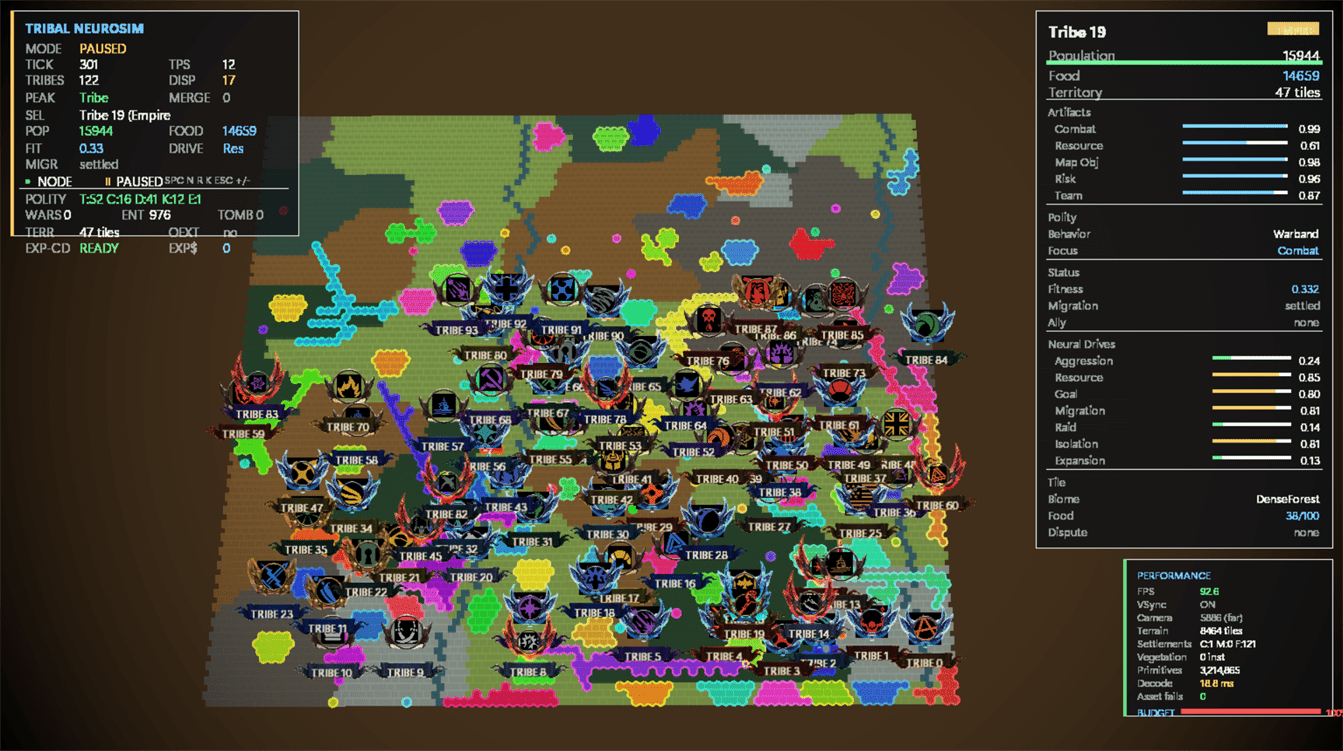
\includegraphics[width=0.9\textwidth]{assets/neurosim/run67sq7777-sq-s7777-tick301-firstempire.png}
\caption{SoloQ, seed=7777, tick=301: az első Empire, Tribe 19, Warband / Combat profillal.}
\label{fig:neurosim-run-sq7777-firstempire}
\end{figure}

\begin{figure}[h]
\centering
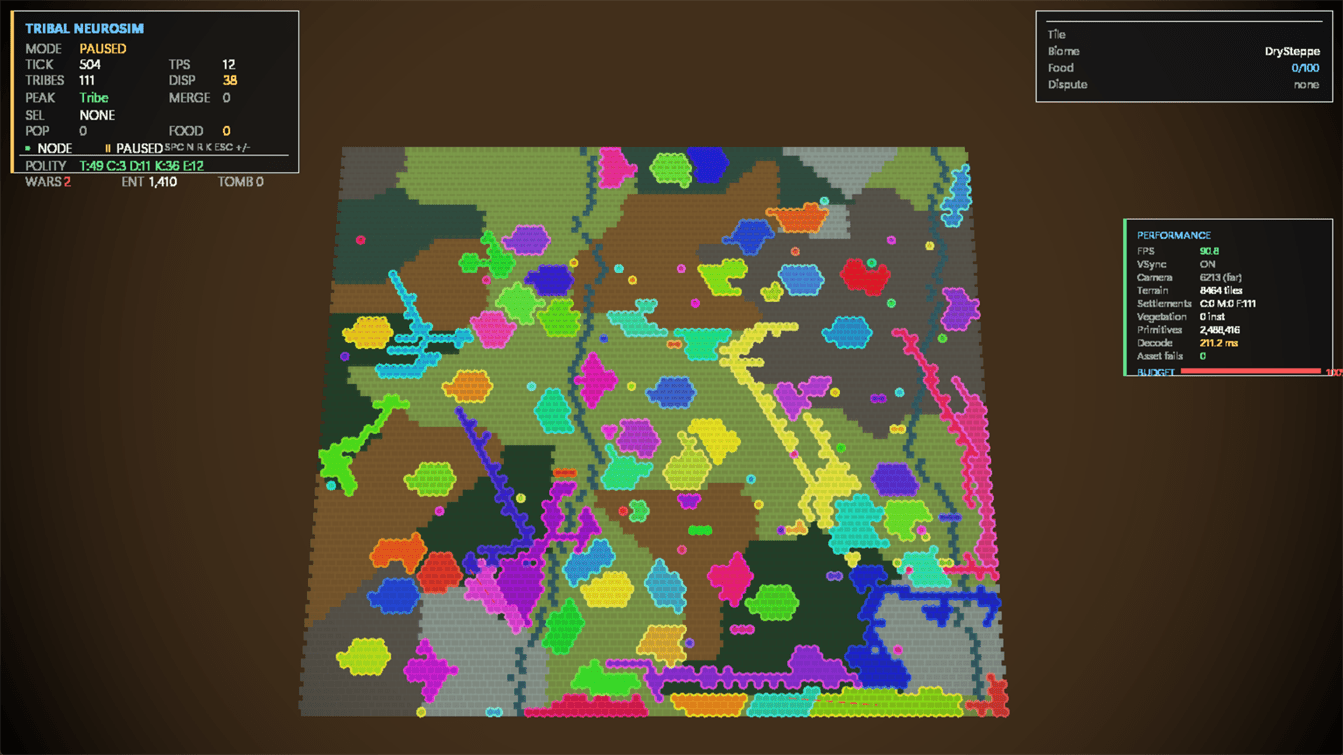
\includegraphics[width=0.9\textwidth]{assets/neurosim/run67sq7777-sq-s7777-tick500.png}
\caption{SoloQ, seed=7777, tick=500: 111 túlélő, még jelentős elválasztott területi foltokkal.}
\label{fig:neurosim-run-sq7777-tick500}
\end{figure}

\begin{figure}[h]
\centering
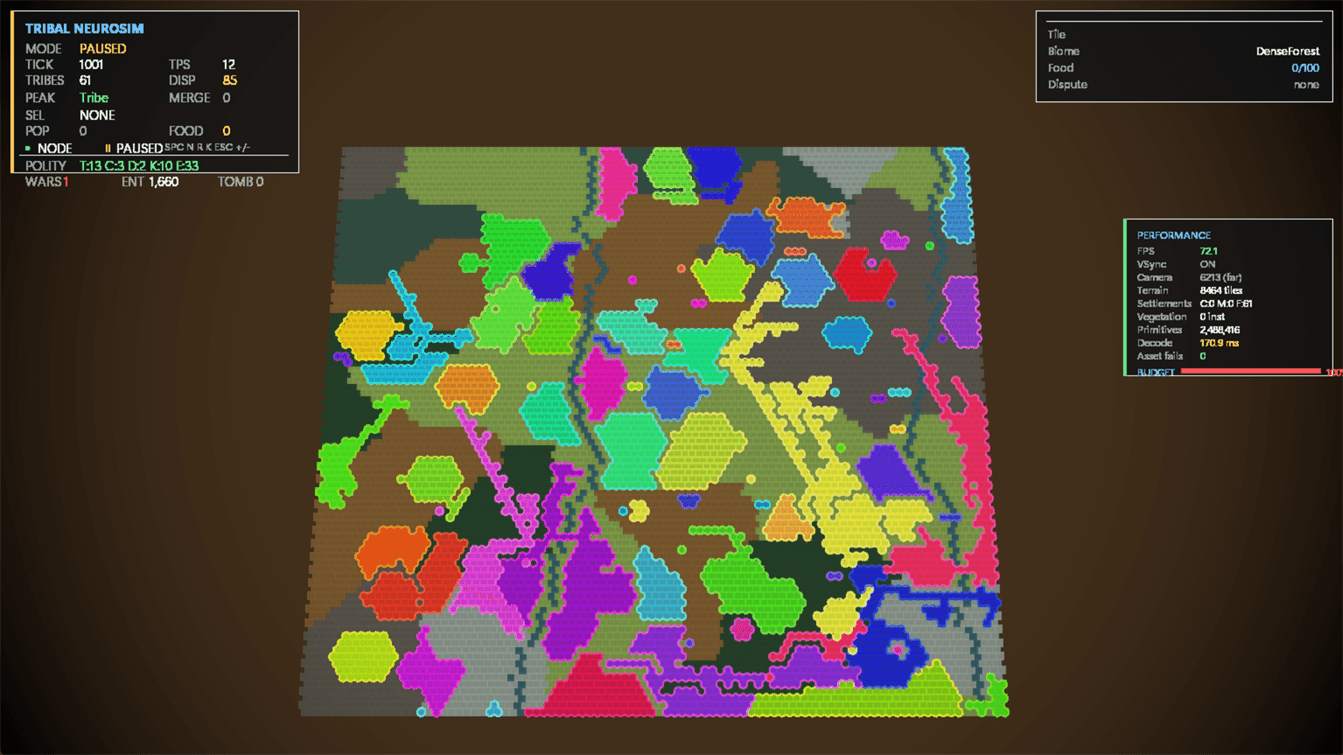
\includegraphics[width=0.9\textwidth]{assets/neurosim/run67sq7777-sq-s7777-tick1000.png}
\caption{SoloQ, seed=7777, tick=1000: 61 túlélő, 33 Empire; a középső stagnáció előtti állapot.}
\label{fig:neurosim-run-sq7777-tick1000}
\end{figure}

\begin{figure}[h]
\centering
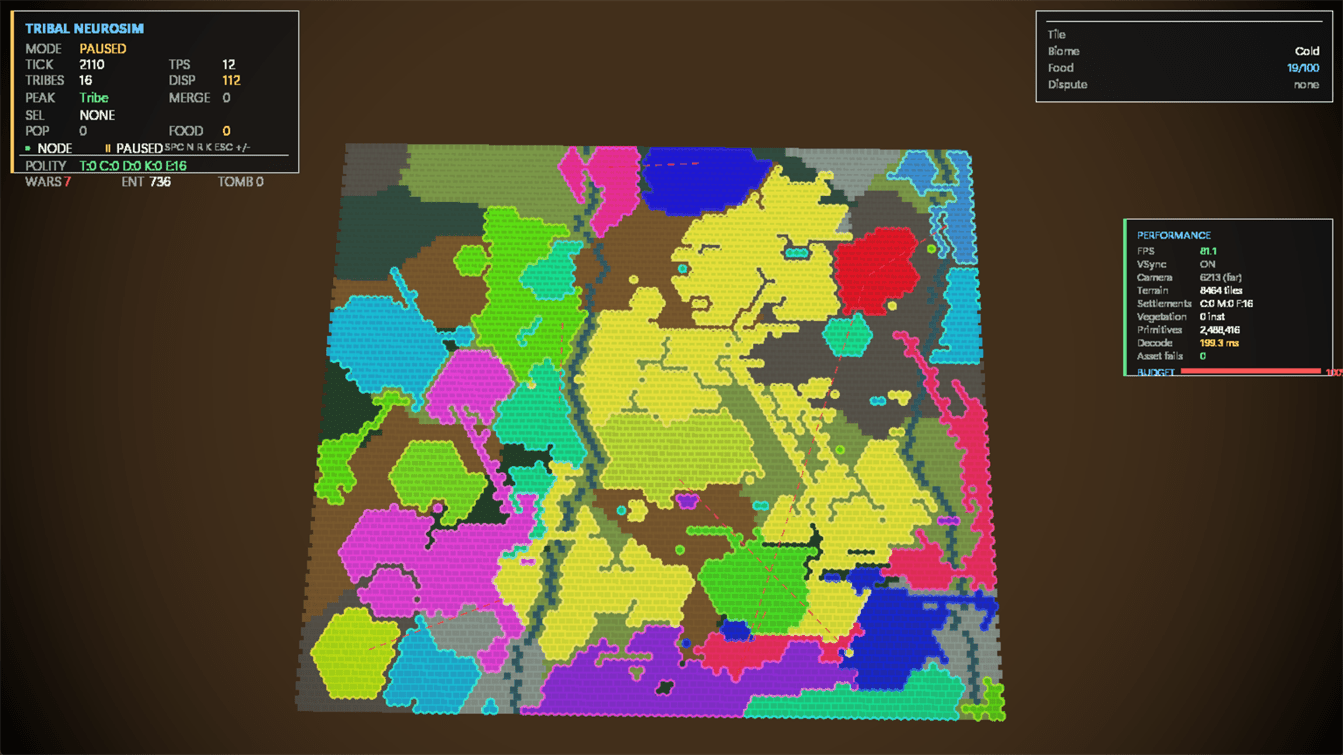
\includegraphics[width=0.9\textwidth]{assets/neurosim/run67sq7777-sq-s7777-tick2100-totalwar.png}
\caption{SoloQ, seed=7777, tick=2110: a tick=2100-as Total War utáni állapot, 18 túlélővel és 7 aktív háborúval.}
\label{fig:neurosim-run-sq7777-totalwar}
\end{figure}

\begin{figure}[h]
\centering
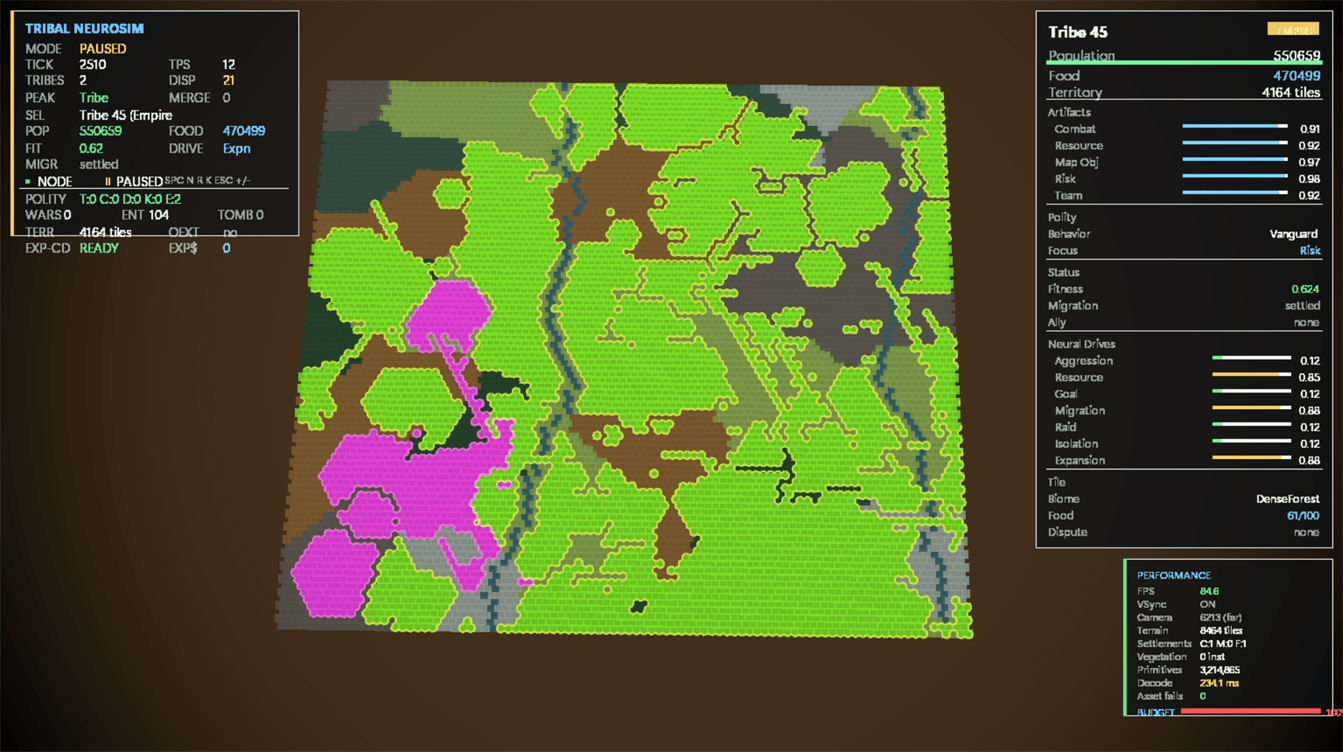
\includegraphics[width=0.9\textwidth]{assets/neurosim/run67sq7777-sq-s7777-tick2510-last2A.png}
\caption{SoloQ, seed=7777, tick=2510: végső két szereplő, Tribe 45 Vanguard / Expansion profillal.}
\label{fig:neurosim-run-sq7777-last2a}
\end{figure}

\begin{figure}[h]
\centering
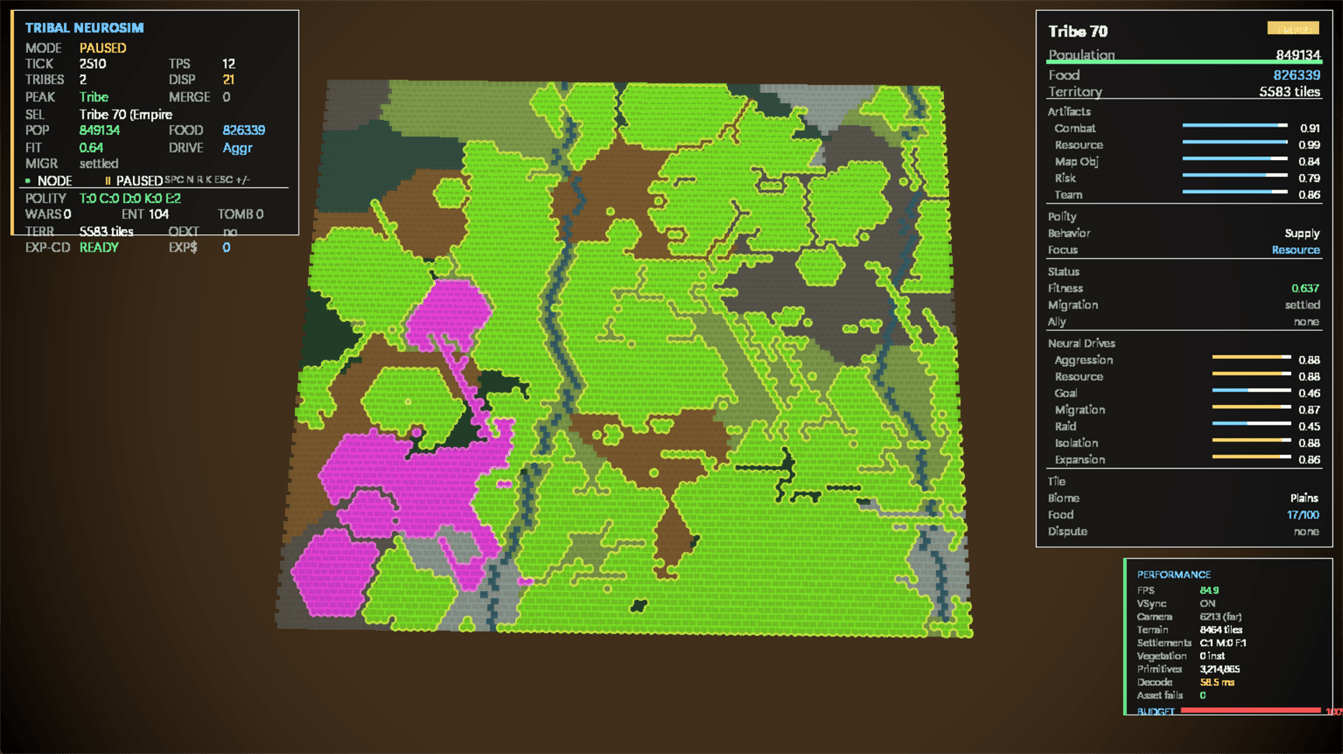
\includegraphics[width=0.9\textwidth]{assets/neurosim/run67sq7777-sq-s7777-tick2510-last2B.png}
\caption{SoloQ, seed=7777, tick=2510: végső két szereplő, Tribe 70 Supply / Resource profillal.}
\label{fig:neurosim-run-sq7777-last2b}
\end{figure}

\begin{figure}[h]
\centering
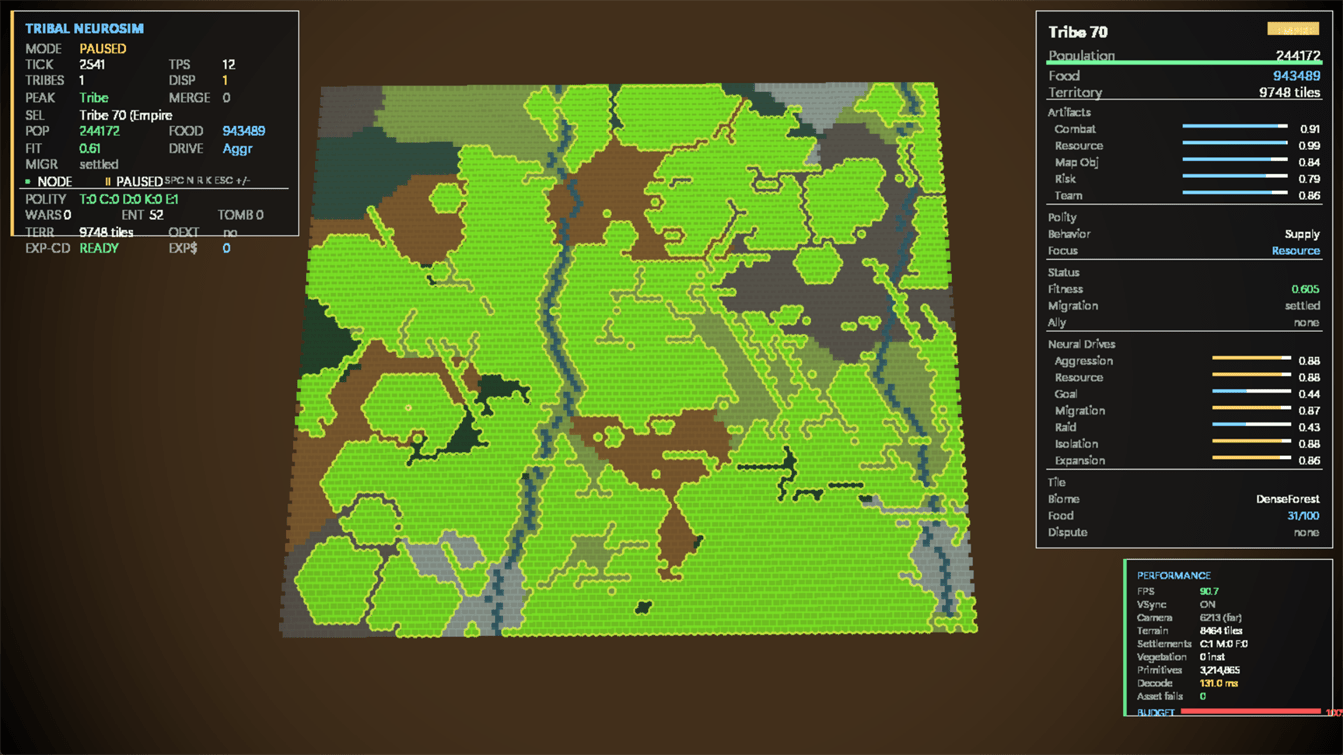
\includegraphics[width=0.9\textwidth]{assets/neurosim/run67sq7777-sq-s7777-tick2541-last.png}
\caption{SoloQ, seed=7777, tick=2541: Tribe 70 győzelme, 9\,748 tile-os végső területtel.}
\label{fig:neurosim-run-sq7777-last}
\end{figure}

% ==========================================================================
\section{Kisebb törzsek győzelme nagyobb entitások felett}
\label{sec:neurosim-26-upset}
% ==========================================================================

A négy futtatás eseménynaplóiban többször megfigyelhető egy első ránézésre
meglepő jelenség: egy, a domináns entitásnál területileg, populációban
és erőforrásokban jelentősen kisebb törzs képes azt legyőzni és abszorbeálni.
A flexset seed=42 futtatásban Tribe~596 kevesebb területtel rendelkezett, mint
Tribe~557, mégis megnyerte a háborút tick=2424-nél. A SoloQ seed=7777 futtatásban
Tribe~45 legyőzte a tartósan domináns Tribe~99-et tick=2340-nél.

Ennek mechanikai magyarázata három tényező kombinációja.

\textbf{Felhalmozott $A\_\text{combat}$ előny.} Az $A\_\text{combat}$ artifaktum minden megnyert
védelmi háborúval növekszik, de csak a ténylegesen megnyert harci körök után.
Egy kis törzs, amelyik több védelmi háborút nyert, magasabb $A\_\text{combat}$-tal
rendelkezhet, mint egy nagy törzs, amelyik expanzióval, nem harccal növekedett.
A Poisson-veszteség képletéből következően ez a különbség non-lineárisan hat:
ha $a_{\text{kis}} > a_{\text{nagy}}$, a kis törzs várható vesztesége alacsonyabb
tick-enként, még ha kontaktzónája kisebb is.

\textbf{Kétfrontos nyomás.} Ahogy a 25.4.~alszakasz tárgyalja, a domináns entitás
egyszerre több szomszéddal kerülhet háborúba. Ha két kisebb törzs egymástól
függetlenül ugyanazon tickben indít háborút a nagyobb ellen (mint a trilaterális
esetben), a Poisson-veszteség mindkét fronton akkumulálódik. A nagy törzs
populációja és élelmiszer-készlete egyszerre csökken, miközben csak az egyik
ellenfelet tudja visszaverni.

\textbf{Erőforrás-szűkösség.} A nagy törzs magas territory fenntartási költsége
és a háborús állapotban szünetelő élelmiszer-gyűjtés (starvation cascade jelenség,
ld. 26.2.~alszakasz) fokozatosan csökkenti a harci kapacitást. Egy kisebb, mobilis
ellenfél számára ez ablakot nyit: a nagy törzs katonailag még erős, de logisztikailag
sérülékeny.

A szimuláció tehát nem biztosítja a méretarányos fölényt. A méret
előny az erőforrástermelésben és a területi jelenlétben, de hátrány a
kétfrontos nyomással szemben és a logisztikai kitettségben. Ez a dinamika
teszi a végső szakaszt nehezen előrejelezhetővé, és hozzájárul ahhoz, hogy
a futtatási narratívák genuinisan emergensnek hatnak.

% ==========================================================================
\section{Adatkészlet-összehasonlítás és értelmezési határok}
\label{sec:neurosim-26-conclusions}
% ==========================================================================

A négy validált Tribal NeuroSim futtatás közös értelmezése nem egyetlen győztes archetípus abszolút fölényéről szól, hanem arról, hogy eltérő adatkészletből származó klaszterpriorok azonos szimulációs szabályok alatt eltérő emergáló stratégiákat hoztak létre. A flexset és a soloq futtatások ugyanazt a szimulációs magot, azonos döntési logikát és determinisztikus seedelést használtak; a különbség a kezdeti klaszterprofilokban és az azok mögött álló gráfstruktúrában volt.

\subsection*{Összefoglaló táblázat}

\begin{table}[h]
\centering
\small
\caption{A négy záró Tribal NeuroSim futtatás összehasonlítása}
\label{tab:neurosim-run-comparison-final}
\resizebox{\textwidth}{!}{%
\begin{tabular}{llllllll}
\hline
\textbf{Futtatás} & \textbf{Adatkészlet} & \textbf{Seed} & \textbf{Győztes} & \textbf{Viselkedés} & \textbf{Agresszió} & \textbf{Migráció} & \textbf{Végső tick} \\
\hline
run67fl7777 & Flexset & 7777 & Tribe 355 & Warband/Combat & 0{,}18 & 0{,}88 & 2538 \\
run67fl42 & Flexset & 42 & Tribe 596 & Warband/Combat & 0{,}13 & 0{,}87 & 2487 \\
run67sq42 & SoloQ & 42 & Tribe 89 & Vanguard/Risk & 0{,}11 & 0{,}16 & 2046 \\
run67sq7777 & SoloQ & 7777 & Tribe 70 & Supply/Resource & 0{,}68 & 0{,}87 & 2541 \\
\hline
\end{tabular}
}
\end{table}

\begin{figure}[h]
\centering
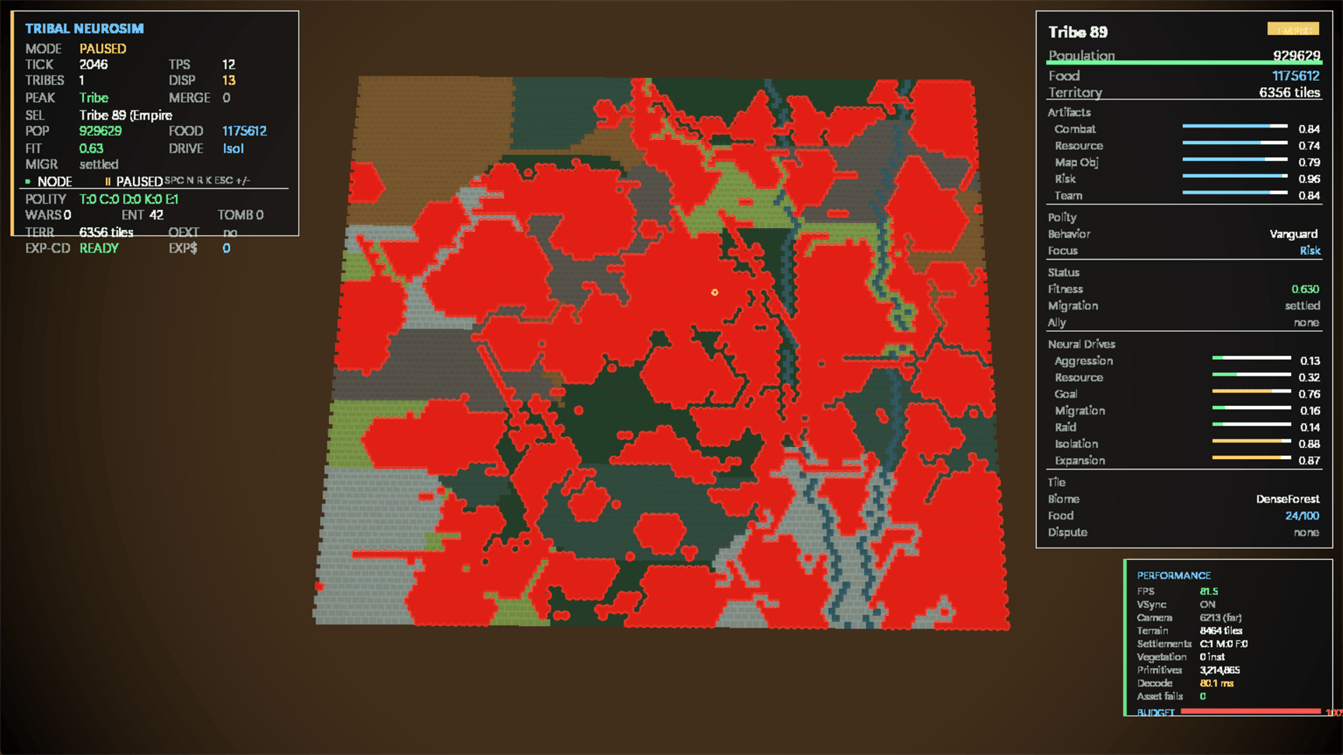
\includegraphics[width=0.9\textwidth]{assets/neurosim/run67sq42-sq-s42-tick2046-last.png}
\caption{SoloQ, seed=42, tick=2046: Tribe 89, Vanguard/Risk, 6\,356 tile}
\label{fig:neurosim-final-sq42}
\end{figure}

\begin{figure}[h]
\centering
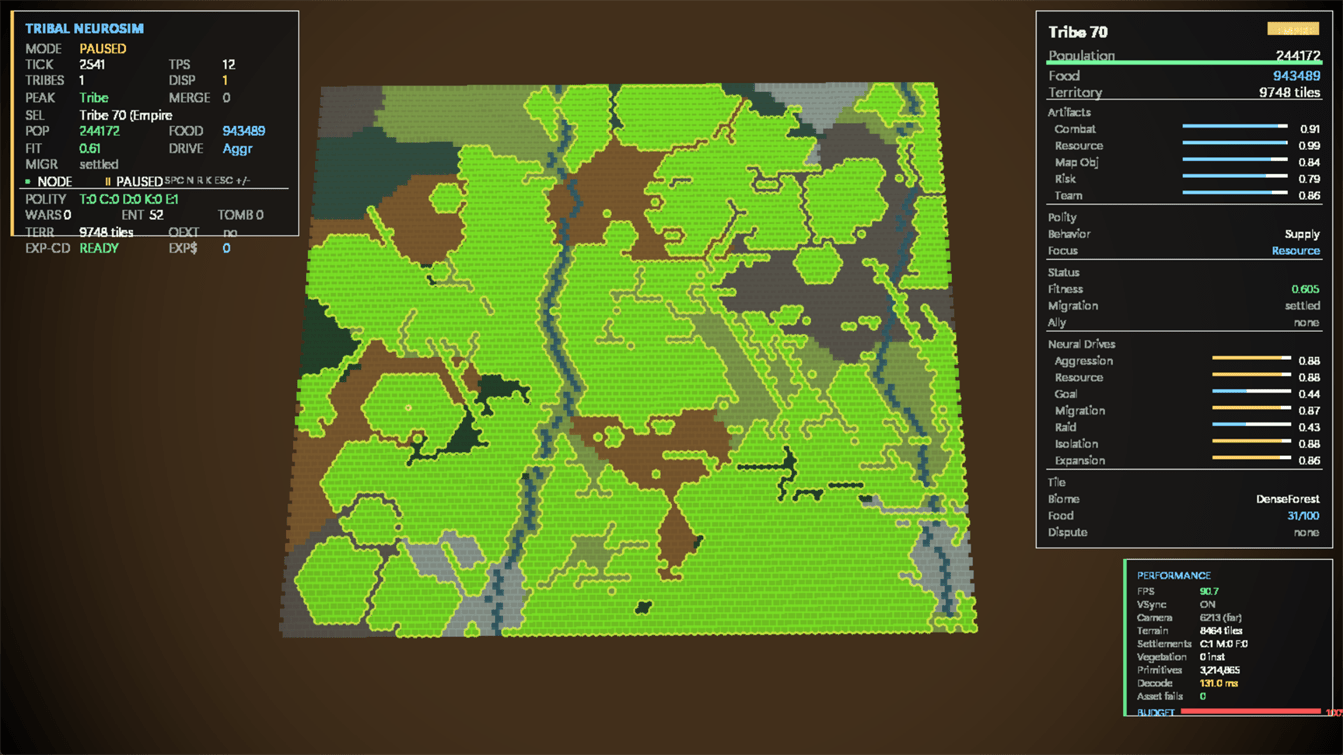
\includegraphics[width=0.9\textwidth]{assets/neurosim/run67sq7777-sq-s7777-tick2541-last.png}
\caption{SoloQ, seed=7777, tick=2541: Tribe 70, Supply/Resource, 9\,748 tile}
\label{fig:neurosim-final-sq7777}
\end{figure}

\subsection*{Győztes archetípus-eloszlás és variabilitás}

A négy kísérleti futtatást egy 103 seed alapú soloq sweep egészíti ki, amely a kisebb (140 törzses) adatkészleten statisztikailag érdemi mintán vizsgálja a győztes archetípusok eloszlását. A sweep minden futtatása Empire polity-szintű győztessel zárult (103/103). Az archetípus-eloszlás:

\begin{table}[H]
\centering
\caption{Győztes archetípus-eloszlás a soloq 103-seed sweep alapján}
\label{tab:soloq-sweep-archetypes}
\begin{tabular}{lrr}
\toprule
\textbf{Archetípus} & \textbf{Futtatások} & \textbf{Arány} \\
\midrule
Warband   & 36 & 35{,}0\% \\
Supply    & 23 & 22{,}3\% \\
Council   & 20 & 19{,}4\% \\
Vanguard  & 14 & 13{,}6\% \\
Pathfinders & 10 & 9{,}7\% \\
\midrule
\textbf{Összesen} & 103 & 100\% \\
\bottomrule
\end{tabular}
\end{table}

Az átlagos befejezési tick 2308{,}57; az átlagos győztes terület 8\,338 tile. A leggyakoribb győztes klaszter 6 alkalommal fordult elő; a leggyakoribb győztes törzs-ID szintén 6 alkalommal szerepelt. Ez \emph{mixed convergence} képet mutat: a Warband archetípus enyhe pluralitással vezet (35\%), de nem rendelkezik erős, seed-független dominanciával.

A SoloQ futtatások tehát nem konvergálnak egyetlen archetípusra. Seed=42 mellett Tribe 89 Vanguard/Risk profillal nyert, alacsony agressziós és alacsony migrációs végállapottal; seed=7777 mellett Tribe 70 Supply/Resource profillal, magasabb agresszióval és magas migrációval zárta a futtatást. A két SoloQ győztes neurális profilja eltért egymástól, és az A\_combat felhalmozódási mintájuk sem ugyanazt a pályát követte: a seed=42 futtatásban a döntő szerep a védelmi túléléshez és célzott kockázatvállaláshoz kötődött, míg a seed=7777 futtatásban a resource-központú túlélés és az endgame-ben megnyíló opportunista ablak volt meghatározó. A 103-seed sweep ezt a képet megerősíti: a soloq változékony győztes-profilt produkál.

A két tesztelt flexset futtatás (seed=42 és seed=7777) ezzel szemben ugyanarra az archetípusra futott ki: mindkét esetben Warband/Combat profilú entitás győzött alacsony agresszióval (0{,}13--0{,}18) és magas migrációval (0{,}87--0{,}88). Ez konzisztens mintázat a vizsgált seedeken, bár a flexset szisztematikus sweepje még nem készült el.

Ez a különbség a mögöttes gráfstruktúrából értelmezhető. A flexset adatkészlet szervezettebb, ismétlődő kapcsolatmintákat hordoz, míg a soloq adatkészlet inkább egyéni teljesítményprofilokat rögzít tartós co-queue struktúra nélkül. A szimulációs eltérés ezért nem pusztán seed-zajként, hanem a klaszterpriorok eltérő szerkezetének következményeként olvasható.

\subsection*{Értelmezési keret}

A Flex Queue klaszterek koordinált csapatjátékot kódolnak. A flexset gráfban az alliance jellegű minták, a komplementer szerepek és az ismétlődő co-queue kapcsolatok nem egyetlen játékos izolált teljesítményét, hanem visszatérő együttjátszási struktúrákat írnak le. Amikor ezekből klaszterprofilok készülnek, a szimuláció olyan entitásokat inicializál, amelyekben a harci kompetencia, a területi önfenntartás és a magas izoláció egyszerre jelenhet meg. A két tesztelt flexset futtatás Warband/Combat kimenetele ebben az értelmezésben nem azt jelenti, hogy ez a profil objektíven jobb minden környezetben, hanem azt, hogy a vizsgált két seednél ez a szabálykörnyezet és klaszterezési struktúra ezt a győztes profilt hozta létre.

A SoloQ klaszterek más jellegű információt hordoznak. Ezek nem tartós társas csapatstruktúrát, hanem rangsorolt egyéni teljesítményprofilokat sűrítenek. A SoloQ inicializáció ezért kevésbé ad át olyan koordinált társas mintát, amely több seed alatt is ugyanabba a túlélési stratégiába húzná a rendszert. Ennek megfelelően a seed=42 futtatás Vanguard/Risk, a seed=7777 futtatás Supply/Resource győztest produkált, vagyis a szimulált kimenet változékonyabb lett.

Az értelmezés korrelatív, nem okozati. Ahogy a 24.3.~alszakasz validációs megfogalmazása is hangsúlyozza, a determinisztikus és esemény-alapon visszaellenőrizhető futtatás azt igazolja, hogy adott klaszterpriorok mellett milyen szimulált dinamika jött létre. Nem igazolja, hogy a valódi játékosok pszichológiai értelemben így viselkednének, és nem állít elő közvetlen LoL-meccs-előrejelzést.

\subsection*{Kiegészítő megfigyelések}

A SoloQ futtatásokban megjelent egy olyan minta, amely a flexset futtatásokból hiányzott: a domináns középső aktor. A SoloQ seed=7777 futtatásban Tribe 99 hosszú középső szakaszon át front-runnerként viselkedett, hét háborút nyert, majd tick=2340-nél mégis kiesett. Ez tiszta narratív ívet adott a futtatásnak: domináns szereplő, többfrontos nyomás, bukás, majd egy másik entitás győzelme. A flexset futtatásokban ezzel szemben a konszolidáció elosztottabb volt, több nagy szereplő párhuzamos nyomásával és kevésbé egyetlen központi midgame-hatalom köré szerveződve.

A futási sebesség értelmezésénél a térképméretet külön kell kezelni. A SoloQ seed=42 futtatás volt a leggyorsabb, tick=2046-os végállapottal, de ez nem önmagában SoloQ-tulajdonság. A futtatás kisebb, körülbelül 7000 tile-os térképen zajlott, ezért a kontaktus, a területi telítődés és a végső konszolidáció hamarabb következhetett be. A gyorsaság tehát részben térszubsztrátum-hatás, nem közvetlen adatkészlet-minősítés.

A Total War skála arányosabb képet ad, ha az indítótörzsek számához viszonyítjuk. A flexset futtatások 599 törzzsel indultak, és a nagy opportunista háborús burstök 55--72 deklarációs nagyságrendben jelentek meg. A SoloQ futtatások 140 törzzsel indultak, és a Total War események 15--17 deklarációs tartományban maradtak. Ez abszolút értékben kisebb, de a mezőny méretéhez viszonyítva továbbra is jelentős konfliktuskoncentrációt jelent.

\subsection*{Amit az eredmény alátámaszt, és amit nem}

Az eredmények alátámasztják, hogy a klaszter-derivált priorok mérhetően eltérő szimulált viselkedést produkálnak azonos szabálykörnyezetben. A flexset, mint koordináltabb gráfstruktúra, a két tesztelt seed alatt konvergens Warband/Combat kimenetelhez vezetett. A soloq, mint inkább egyéni teljesítményprofilokat hordozó adatkészlet, változékonyabb győztes archetípusokat produkált. A négy futtatás reprodukálható, inspektálható és esemény-alapon igazolt: a következtetések nem kizárólag a végső képernyőképekből, hanem a háborús, terjeszkedési és eliminációs események naplózott sorozatából származnak.

Az eredmények ugyanakkor nem bizonyítanak valódi játékos-pszichológiát. Nem állítják, hogy a Flex Queue játékosok szükségszerűen Warband-szerűen, a SoloQ játékosok pedig Vanguard- vagy Supply-szerűen viselkednek. Nem adnak előrejelzést tényleges League of Legends meccsek kimenetelére, és nem bizonyítják a Warband/Combat archetípus objektív fölényét. A Warband/Combat itt szimulációs környezetben, adott gráf-derivált priorok és adott szabályrendszer alatt megfigyelt túlélési stratégia, nem általános játékelméleti optimum.

A legerősebb thesis-szintű következtetés ezért határkijelölő: a Tribal NeuroSim nem feketedobozos igazsággép, hanem ellenőrizhető transfer-kísérlet. Megmutatja, hogy a PremadeGraph-ból származó klaszterprofilok viselkedési priorokká alakíthatók, ezek evolúciós többügynökös környezetben futtathatók, és az eredmények eseményszinten visszavezethetők a szimulációs dinamikára. Az oksági állítás azonban nyitva marad: a futtatások nem bizonyítják, hogy az adatkészlet-struktúra közvetlenül okozza a győztes archetípust, csak azt, hogy a különböző struktúrából származó priorok ebben a rendszerben különböző kimenetekkel társultak.

A Tribal NeuroSim szimulációiban a végső győztes az összes tile-t, az összes erőforrást és az
összes leszármazási vonalat örökli. Nincs részleges kimenetel, nincs megosztott
győzelem, nincs béke. A rendszer így alkalmas eszköz az evolúciós szelekciós
nyomás vizsgálatára: a szabályrendszer minden esetben egyértelmű, ellenőrizhető
és reprodukálható eredményt kényszerít ki.

A Tribal NeuroSim demonstrálja, hogy eltérő szociális hálózati struktúrákból -- szervezett Flex Queue csapatokból versus egyéni SoloQ rangsorolt játékosoktól -- származó, gráf-derivált klaszterprofilok mérhetően eltérő emergáló túlélési stratégiákat produkálnak, amikor azonos szabályok alatt evolúciós többügynök-szimulációba kerülnek. A flexset adatkészlet mindkét tesztelt seednél alacsony agressziójú Warband/Combat győztest hozott; a soloq 103-seed sweep mixed convergence-t mutat, Warband enyhe pluralitással (35\%), de erős seed-független dominancia nélkül. Ez a viselkedési különbség a mögöttes gráfstruktúra tükröződéseként értelmezhető, nem valódi teljesítmény-fölény bizonyítékaként.

\bigskip

% ==========================================================================
\section{Jövőbeli alkalmazások és transzfer-lehetőségek}
\label{sec:neurosim-26-future}
% ==========================================================================

A Tribal NeuroSim elsősorban League of Legends játékos-klaszterprofilokkal
validált rendszer, de a szimulációs architektúra és az artifact-prior mechanizmus
nem LoL-specifikus. Ebben a szekcióban néhány olyan területet vázolok, ahol
a rendszer ugyanolyan módszertannal alkalmazható lenne.

\subsection*{A leképezhető artifact-priorok általánosítása}

Az öt artifact (\textit{A\_combat}, \textit{A\_resource}, \textit{A\_map\_objective},
\textit{A\_risk}, \textit{A\_team}) nem más, mint öt normált teljesítménymutatóból
álló vektor. Bármilyen domain, ahol hasonló dimenziók értelmezhetők, potenciális
transzfer-forrás:

\begin{itemize}
  \item \textbf{Csapatsportok és e-sportok.} Egy kosárlabda-csapat vagy Counter-Strike
    klán statisztikáiból (harci = fragtörténet, resource = gazdasági döntések, map = pozícionálás,
    risk = pushok vállalása, team = asszisztok és clutch-mentések) ugyanolyan klaszterprofilok
    képezhetők. A szimulációban az ilyen csapatprofilok versenyeznek erőforrásokért és
    területért, és az eredmény statisztikailag összevethető a valódi kiesési arányokkal.
  \item \textbf{Startupok és üzleti szervezetek.} Egy vállalat növekedési profilja
    (expanziós aggresszivitás, erőforrás-hatékonyság, piaci célzás, kockázattűrés,
    csapatkoordináció) leképezhető az öt artifaktra. A szimuláció ilyenkor piaci
    versenykörnyezetként viselkedik, és megfigyelhető, hogy adott profilkombinációk
    milyen körülmények között dominálnak.
  \item \textbf{Ökológiai populációdinamika.} Az $A\_\text{combat}$ $\leftrightarrow$ predációs képesség,
    $A\_\text{resource}$ $\leftrightarrow$ táplálékkeresési hatékonyság, $A\_\text{risk}$ $\leftrightarrow$ migrációs kockázatvállalás,
    $A\_\text{team}$ $\leftrightarrow$ koloniális koordináció (pl. falkák, hangyák). A hex-rács biome-rendszere
    ökológiai térképre vetítve egy vizsgálható populációdinamikai szimulátort ad.
  \item \textbf{Katonai szimulációk és hadijáték-elemzés.} A területi mechanika,
    a kétfrontos nyomás és a Poisson-harci modell közelebb áll a Lanchester-féle
    harcmodellhez \cite{lanchester1916}, mint ahogy azt a LoL-kontextus sugallja.
    Valódi katonai egységadatokra vetítve az architektúra közvetlen policy-szimulációs
    eszközként is használható.
\end{itemize}

\subsection*{Módszertani transzferálhatóság}

A PremadeGraph projektben alkalmazott eszközök (gráfklaszterezés, asszortativitási
elemzés, Brandes-féle betweenness centralitás, 3D Bird's Eye Sphere, pathfinder
algoritmusok) szintén nem LoL-specifikusak. Bármilyen hálózatban, ahol csúcsok
közötti kapcsolat meghatározható és teljesítménymutató rendelhető a csúcsokhoz,
ugyanez a pipeline alkalmazható:

\begin{itemize}
  \item Közösségi hálózatok: ki a kulcsszereplő (centralitás), hogyan szegmentálható
    a közösség (klaszterezés), mennyire homofil a kapcsolatstruktúra (asszortativitás)?
  \item Logisztikai hálózatok: optimális útvonal (pathfinder), kritikus csomópontok
    eltávolítási hatása (betweenness centralitás), hierarchikus struktúra vizualizálása
    (3D sphere).
  \item Akadémiai kollaborációs hálózatok: szerzői klaszterek (közösségi struktúra),
    tudásáramlás irányai (irányított gráf asszortativitás), befolyásos közvetítők
    (centralitás).
\end{itemize}

A Riot Games API azért különösen alkalmas prototípus-adatforrás, mert nyilvánosan
elérhető, strukturált és gazdag metaadatokban. De a módszertan nem igényel LoL-adatot:
ugyanolyan pipeline futtatható bármilyen nyílt API-ra (Twitter/X graph API, GitHub
kollaborációs gráf, NBA teljesítmény-adatbázis), ahol hasonló felosztás kivitelezhető.

\subsection*{A neuroevolúciós szimuláció önálló értéke}

A Tribal NeuroSim NeuroEvolution of Augmenting Topologies paradigmával kombinálja az
ABM/MAS architektúrát. Ez a kombináció önmagában is kutatási értéket hordoz:
az NEAT-stílusú kontrollerek lehetővé teszik, hogy a klaszterpriorokból induló
stratégiai viselkedés ne pusztán determinisztikusan öröklődjön, hanem evolúciós
nyomás alatt módosuljon és differenciálódjon. A rendszer ezért nem egyszerű
,,mi lenne ha'' szimulator, hanem egy exploratív evolúciós tér, amelyben az
inicializálási feltételek és a végeredmény közötti kapcsolat empirikusan vizsgálható.
